\documentclass[notheorems,envcountsect,t,xcolor=table,aspectratio=169]{beamer}
\synctex=1
%draft
%\includeonlyframes{bib,current}
%,notes=show
%,hyperref={bookmarks=true}
%trans
%beamer
%handout
%notes=hide/show/only

%\usepackage[usenames,dvipsnames]{xcolor}

%\newcommand{\nop}[1]{}
\newcommand{\nop}[1]{#1}
\usepackage{enumerate}

\usepackage[usestackEOL]{stackengine} % to use \Longstack
\usepackage{pifont}% http://ctan.org/pkg/pifont
\newcommand{\cmark}{\ding{51}}%
\newcommand{\xmark}{\ding{55}}%

\usepackage{array,etoolbox}
\preto\tabular{\setcounter{magicrownumbers}{-1}}
\newcounter{magicrownumbers}
\newcommand\rownumber{\stepcounter{magicrownumbers}\arabic{magicrownumbers}}

% TABLE EXTRAS
\usepackage{array}
\newcolumntype{H}{>{\setbox0=\hbox\bgroup}c<{\egroup}@{}}
\newcommand{\ts}[1]{\textit{#1}}
\newcommand{\tm}[1]{\textbf{#1}}


%fix to many includes
%"! No room for a new \dimen"
\usepackage{etex}


	\usepackage{listings}
	\usepackage{tikz}
	\usepackage{color}
	%\usepackage{soul}
	%\usepackage{adjustbox}
	\usepackage{colortbl}
	\usepackage{multicol}
	\usepackage{multirow}  % Allows table elements to span several rows.
	\usepackage{booktabs}  % Improves the typesettings of tables.

	%\usepackage{floatrow}
	% Table float box with bottom caption, box width adjusted to content
	%\newfloatcommand{capbtabbox}{table}[][\FBwidth]
	\newcommand{\blahtab}[1]{{\tiny{#1}}}%
	%\usepackage{blindtext}
	\newcommand{\parhead}[1]{\smallskip\noindent\textbf{#1}\ }				

	%\usepackage{memoir}
	%\usepackage{appendixnumberbeamer}
	%>>>
	%<<< Set up listings

	\newcommand{\inputPredColor}{purple!70!black}
	\newcommand{\outputPredColor}{orange!70!black}
	\newcommand{\specialTermColor}{blue!70!black}
	\definecolor{dkgreen}{rgb}{0,0.5,0}
	%\setstcolor{\specialTermColor}
	%\setstcolor{\specialTermColor}
	%\sethlcolor{\specialTermColor}
	\definecolor{gyellow}{rgb}{1.0, 0.97, 0.33}
	\definecolor{mygreen}{RGB}{0,192,0}
	\definecolor{myblue}{RGB}{40,40,255}
	\definecolor{myorange}{RGB}{253,126,0}

	\definecolor{HighlightColor}{rgb}{1.0, 0.97, 0.33}
	%\definecolor{HighlightColor}{rgb}{1.0, 0.5, 0}
	%\definecolor{HighlightColor}{rgb}{0.13,0.67,0.8}
	\makeatletter
	\def\rowcolor{\noalign{\ifnum0=`}\fi\bmr@rowcolor}
	\newcommand<>{\bmr@rowcolor}{%
	    \alt#1%
		{\global\let\CT@do@color\CT@@do@color\@ifnextchar[\CT@rowa\CT@rowb}% 
		{\ifnum0=`{\fi}\@gooble@rowcolor}% 
	}

	\newcommand{\@gooble@rowcolor}[2][]{\@gooble@rowcolor@}
	\newcommand{\@gooble@rowcolor@}[1][]{\@gooble@rowcolor@@}
	\newcommand{\@gooble@rowcolor@@}[1][]{\ignorespaces}
	\makeatother

	\newcommand{\predicate}[1]{\texttt{\small #1}}

	\lstdefinelanguage{dflat}{
	    firstnumber=1, % XXX Workaround because otherwise warnings occur with hyperref
	    otherkeywords={:-},
	    morekeywords={not},
	    keywordstyle=\sffamily\bfseries,
	%    emph={root,childNode,current,introduced,removed,childRow,sub,childItem,childCount,childCost,item,extend,count,cost,currentCost,levels,optItem},
	    emph={final,childNode,current,introduced,removed,childRow,sub,childItem,childCount,childCost,childAuxItem,bag, atNode, rootOf, root},
	    moreemph=[2]{item,extend,count,cost,currentCost,levels,optItem,auxItem , reject, accept, or, and, length},
	    moreemph=[3]{pos, neg, att, head, p, clause, atom, z, sim, cor,minimize, fix},
	    moreemph=[4]{},%out, in, outc, def, defc},
	    alsoletter={\#}, % This is required to avoid coloring, e.g., the #count aggregate because it is mistakenly interpreted as the count/1 predicate
	%    emphstyle=\rmfamily,
	%    emphstyle=[2]\slshape,
	    emphstyle=\color{\inputPredColor},
	    emphstyle=[2]\color{\outputPredColor},
	    emphstyle=[3]\color{\specialTermColor},
	    emphstyle=[4]\color{\decompositionColor},
	    morecomment=[l]{\%},
	    commentstyle=\rmfamily\small\itshape\color{dkgreen},
	    %numbers=left,
	    numbersep=1pt,                  % how far the line-numbers are from the code
	    numberstyle=\tiny\color{gray},
	    numberblanklines=false,
	   % flexiblecolumns=true,
	    %columns=fullflexible,
	%    lineskip=1mm,
	    literate={:-}{{$\la$}}2 {!=}{{$\neq$}}1,
	    breakindent=20pt,
	    escapechar=@, % Useful, e.g., for manually breaking lines via @\\@
	}
	\lstset{%
		aboveskip=0mm,
		belowskip=0mm,
		basicstyle=\footnotesize\ttfamily,
		tabsize=4,
		breaklines=true,
		breakatwhitespace=true,
		fontadjust,
		language=dflat,
	    %firstnumber=1,%
	}
	%>>>
	%<<< Set up TikZ


\lstdefinelanguage{dflat}{
    firstnumber=1, % XXX Workaround because otherwise warnings occur with hyperref
    otherkeywords={:-},
    morekeywords={not},
    keywordstyle=\sffamily\bfseries,
%    emph={root,childNode,current,introduced,removed,childRow,sub,childItem,childCount,childCost,item,extend,count,cost,currentCost,levels,optItem},
    emph={final,childNode,current,introduced,removed,childRow,sub,childItem,childCount,childCost,childAuxItem,bag, atNode, rootOf, root},
    moreemph=[2]{item,extend,count,cost,currentCost,levels,optItem,auxItem , reject, accept, or, and, length},
    moreemph=[3]{pos, neg, att, head, p, clause, atom, z, sim, cor,minimize, fix},
    moreemph=[4]{},%out, in, outc, def, defc},
    alsoletter={\#}, % This is required to avoid coloring, e.g., the #count aggregate because it is mistakenly interpreted as the count/1 predicate
%    emphstyle=\rmfamily,
%    emphstyle=[2]\slshape,
    emphstyle=\color{\inputPredColor},
    emphstyle=[2]\color{\outputPredColor},
    emphstyle=[3]\color{\specialTermColor},
    emphstyle=[4]\color{\decompositionColor},
    morecomment=[l]{\%},
    commentstyle=\rmfamily\small\itshape\color{dkgreen},
    %numbers=left,
    numbersep=1pt,                  % how far the line-numbers are from the code
    numberstyle=\tiny\color{gray},
    numberblanklines=false,
   % flexiblecolumns=true,
    %columns=fullflexible,
%    lineskip=1mm,
    literate={:-}{{$\la$}}2 {!=}{{$\neq$}}1,
    breakindent=20pt,
    escapechar=@, % Useful, e.g., for manually breaking lines via @\\@
}
\lstset{%
	aboveskip=0mm,
	belowskip=0mm,
	basicstyle=\footnotesize\ttfamily,
	tabsize=4,
	breaklines=true,
	breakatwhitespace=true,
	fontadjust,
	language=dflat,
    %firstnumber=1,%
}
%>>>
%<<< Set up TikZ
\usetikzlibrary{arrows,automata,shapes,calc,shadows,positioning,fit,decorations.pathreplacing}
%\usetikzlibrary{external}
%\tikzexternalize[prefix=external-figures/]

%http://tex.stackexchange.com/questions/117873/add-a-curved-arrow-and-a-bracket-to-a-table
\newcommand{\tikzmark}[2][-3pt]{\tikz[remember picture, overlay, baseline=-0.5ex]\node[#1](#2){};}
\newcounter{arrow}
\setcounter{arrow}{0}
\newcommand{\drawcurvedarrow}[3][]{%
 \refstepcounter{arrow}
 \tikz[remember picture, overlay]\draw (#2.center)edge[#1]node[coordinate,pos=0.5, name=arrow-\thearrow]{}(#3.center);
}

\tikzstyle{cc}=[color=red,thin,->,>=to]
\tikzstyle{tdnode} = [draw,rounded corners,minimum size=1.1em, font=\small, prefix after command={\pgfextra{\tikzset{every label/.style={font=\small, label distance=-0.1cm}}}},
left color=blue!10!gray!10, right color=blue!30!gray!10, middle color=white]
\tikzstyle{tdedge} = [-,thick]
\tikzstyle{itemtreed1} = [level 1/.style={sibling distance = 3.7em}, level distance = 2.0em]
\tikzstyle{itemtreed1small} = [level 1/.style={sibling distance = 2.7em}, level distance = 2.9em]
\tikzstyle{itemtree} = [level 1/.style={sibling distance = 5.1em}, level 2/.style={sibling distance = 3.3em}, level distance = 2em]
\tikzstyle{itrootnode} = [draw,circle, minimum size=0.4em, left color=white, right color=white, middle color=white]
\tikzstyle{itnode} = [draw,rounded corners,minimum size=1.5em, node distance=0.7em, left color=red!10, right color=red!25, middle color=white]
\tikzstyle{extensionpointer} = [->, densely dashed, scale=0.7]
\tikzstyle{extensionpointerback} = [extensionpointer, <->]
\tikzstyle{counterpointer} = [->, solid, scale=0.7]
\tikzstyle{highlight} = [red,thick]
\tikzstyle{arrowstyle}=[arrowfill, single arrow, inner sep=0.3em, yscale=0.5, single arrow, single arrow head extend=.25em]
\tikzstyle{arrowfill}=[top color=red!50, bottom color=red!80]%, general shadow={fill=black, shadow yshift=-0.8ex, path fading=arrowfading}]
\tikzstyle{coderef}=[fill=white,shape=circle, inner sep=0, outer sep=0, font=\small]%, text=black]
\tikzstyle{argument}=[circle,fill=white,draw=black,thin,minimum size=9mm]
\tikzstyle{ptr}=[draw,rectangle,minimum height=0.25cm,minimum width=0.25cm]
\tikzstyle{extpointer}=[->,dashed,>=latex]

\tikzstyle{gnode} = [draw, circle, node distance=0.2em, inner sep=1.5pt, outer sep=0pt, minimum size=0.8em]%, font=\scriptsize]

\tikzstyle{bddnode} = [draw, rectangle, rounded corners=0.1em, minimum size=1.15em, inner sep=0, font=\scriptsize, left color=yellow!10, right color=yellow!10, middle color=yellow!10]
\tikzstyle{bddepos} = [->,solid]
\tikzstyle{bddeneg} = [->,densely dashed]
\tikzstyle{tdnodetab} = [tdnode,
left color=green!30!gray!10, right color=green!30!gray!10, middle color=green!30!gray!10]

\tikzstyle{rect1} = [fill=blue!30,rounded corners=2pt]
\tikzstyle{rect2} = [fill=blue!10,rounded corners=2pt]
\tikzstyle{rect3} = [gray!60, fill=gray!10, rounded corners=2pt]




%\tikzfading[name=fade south, top color=transparent!0, bottom color=transparent!100]

\tikzset{
	%auto,
	%font=\scriptsize,
	% Cf. http://tex.stackexchange.com/questions/6135/how-to-make-beamer-overlays-with-tikz-node
	onslide/.code args={<#1>#2}{%
		\only<#1>{\pgfkeysalso{#2}}
	}
}

\tikzstyle{subway}=[
	font=\tiny,
	rounded corners=2pt,
	subwayedge/.style={line width=1.4mm},
	u1/.style={subwayedge,draw=red},
	u2/.style={subwayedge,draw=violet},
	u3/.style={subwayedge,draw=orange},
	u4/.style={subwayedge,draw=green!70!black},
	u6/.style={subwayedge,draw=brown},
	station/.style={circle,draw,line width=0.8pt,fill=white, outer sep=0pt, inner sep=3pt},
	smallstation/.style={rectangle, inner sep=0, outer sep=0pt, minimum height=3mm, minimum width=1.5mm, sharp corners},
	u1station/.style={smallstation,fill=red},
	u2station/.style={smallstation,fill=violet},
	u3station/.style={smallstation,fill=orange},
	u4station/.style={smallstation,fill=green!70!black},
	u6station/.style={smallstation,fill=brown},
	sname/.style={inner sep=0pt, outer sep=0pt},
	sname spaced/.style={},
%	solution/.style={draw=black,top color=black,bottom color=black!50,line width=0.8pt,double},
]

\tikzstyle{subwayscaled}=[
	subway,
	scale=0.5,
	every node/.style={transform shape},
	subwayedge/.style={line width=0.7mm},
	station/.style={circle,draw,line width=0.6pt,fill=white, outer sep=0pt, inner sep=3pt},
%	solution/.style={draw=black,top color=black,bottom color=black!50,line width=0.4pt,double},
	solution/.style={},
]

\tikzstyle{subwaytiny}=[
	subway,
	scale=0.4,
	every node/.style={transform shape},
	subwayedge/.style={line width=0.56mm},
	station/.style={circle,draw=black,line width=0.48pt,fill=white, outer sep=0pt, inner sep=3pt},
	solution/.style={},
]

\newcommand{\vertexTopColor}{white}
\newcommand{\vertexBottomColor}{blue!20!black!15}
\tikzstyle{vertex}=[%
	draw,
	circle,
	minimum size=6mm,
	top color=\vertexTopColor,
	bottom color=\vertexBottomColor,
	]
\tikzstyle{tdnode}=[%
	draw,
	rounded corners,
	top color=\vertexTopColor,
	bottom color=\vertexBottomColor,
	]
%>>>
%<<< Macros to use as shortcuts


	\newcommand{\attacks}{\rightarrowtail}
	\renewcommand{\O}{\ensuremath{\mathcal{O}}}
	\renewcommand{\implies}{\ensuremath{\supset}}
	\newcommand{\pred}[1]{\texttt{#1}}
	\newcommand{\problemname}[1]{\textsc{#1}}
	\newcommand{\threeCol}{\problemname{$3$-Col}} % The figure 3 is set in math mode because loading, e.g., mathpazo with the osf option would set the 3 as a text figure (cf. wikipedia) which looks odd in small caps.
	\newcommand{\minCol}{\problemname{Minimal $3$-Coloring}}
	\newcommand{\sat}{\problemname{Sat}}
	\newcommand{\qsat}{\problemname{Qsat}}
	\newcommand{\threeSat}{\problemname{$3$-Sat}}
	\newcommand{\twoSat}{\problemname{$2$-Sat}}
	\newcommand{\hamCycle}{\problemname{Hamiltonian Cycle}}
	\newcommand{\vertexCover}{\problemname{Vertex Cover}}
	\newcommand{\mvc}{\problemname{Minimum Vertex Cover}}
	\newcommand{\cyclicOrdering}{\problemname{Cyclic Ordering}}
	\newcommand{\msoFormulaEvaluation}{\problemname{Mso Formula Evaluation}}
	\newcommand{\mids}{\problemname{Minimum Independent Dominating Set}}
	\newcommand{\complexityclass}[1]{\ensuremath{\mathsf{#1}}}
	\let\defaultP\P
	\renewcommand{\P}{\complexityclass{P}}
	\newcommand{\NP}{\complexityclass{NP}}
	\newcommand{\PH}{\complexityclass{PH}}
	\newcommand{\Pspace}{\complexityclass{PSPACE}}
	\newcommand{\Sp}[1]{\ensuremath{\Sigma^p_{#1}}}
	\newcommand{\Pp}[1]{\complexityclass{\Pi^p_{#1}}}
	\newcommand{\Dp}[1]{\complexityclass{\Delta^p_{#1}}}
	%\newcommand{\co}{\complexityclass{co-}}
	\mathchardef\mhyphen="2D
	\newcommand{\co}{\complexityclass{co\mhyphen}}
	\newcommand{\sizeof}[1]{\ensuremath{\lvert #1 \rvert}}
	\newcommand{\dneg}{\ensuremath{\operatorname{not}\,}}
	\newcommand{\dflat}{\mbox{D-FLAT}}
	\newcommand{\A}{\ensuremath{\mathcal{A}}}
	%\renewcommand{\phi}{\varphi}
	%\newcommand{\undef}{\ensuremath{\textrm{undef}}}


	%\newcommand{\pname}[1]{\mathrm{\rmfamily\scshape #1}} % \textsc{#1}\xspace}
	\newcommand{\pname}[1]{{#1}} % \textsc{#1}\xspace}
	%\newcommand{\problem}[1]{\textsc{#1}}
	\newcommand{\Sat}{\problemname{Sat}}
	\newcommand{\MinSat}{\problemname{$k,\subseteq$-Minimal Sat}}
	\newcommand{\MaxSat}{\problemname{MaxSat}}
	\newcommand{\Circ}{\problemname{Circ}}


\newcommand{\BigO}[1]{\ensuremath{\mathcal{O}(#1)}}
\newcommand{\Card}[1]{|#1|}

\mode<presentation>
{
  % \usetheme{default}
  \usetheme{DRM}
  % \useoutertheme{infolines}
  \usecolortheme{rose}
  \setbeamercolor{block title}{fg=DRMBlue,bg=}

  % \setbeamertemplate{navigation symbols}{}
  \setbeamertemplate{blocks}[rounded]
  %\addtobeamertemplate{block begin}{\pgfsetfillopacity{0.5}}{\pgfsetfillopacity{1}}
  \setbeamertemplate{footline}[frame number]{}
  \setbeamercolor{structure}{fg=blue!40!gray!50!black}
  \setbeamercolor{example text}{fg=green!50!gray!60!black}
  %	\setbeamercolor{block title}{bg=blue!20!gray!25}
  %	\setbeamercolor{block title example}{bg=green!25!gray!40}
}

%\newcommand{\tikzmark}[1]{\tikz[overlay,remember picture] \node (#1) {};}


%===================================================================
%		Basic Stuff
%===================================================================
\usepackage{xspace}
\usepackage{amssymb}% http://ctan.org/pkg/amssymb
\usepackage{amsmath}
\usepackage{mathtools}
\usepackage{url}
\usepackage{xspace}
\usepackage{setspace} 
\usepackage{mathtools}

\newcommand{\F}[1]{F^{\mathit{#1}}}
\DeclareMathAlphabet{\mathpzc}{OT1}{pzc}{m}{it}
\DeclareMathOperator{\width}{width}


\usepackage{bbding}
\usepackage{listings}
\lstset{basicstyle=\ttfamily, escapechar=\%}
%\usepackage{enumitem}

\newcommand{\pvar}[1]{\ensuremath{{\text{#1}}}}
\newcommand{\FSkept}{F_{\text{Caut}}}
\newcommand{\FBrave}{F_{\text{Brave}}}

\newcommand{\eqdef}{\ensuremath{\,\mathrel{\mathop:}=}}
\newcommand{\cid}[1]{\ensuremath{[\![#1]\!]}}
\DeclareMathOperator{\attr}{att}


%===================================================================
%		Algorithms
%===================================================================
%\usepackage[ruled,linesnumbered,noend,noline]{algorithm2e}

\usepackage{cancel}

\usepackage{docmute}
\makeatletter
\newcommand*{\loadpresentation}[1]{{\beamer@inlecturefalse\input{#1}}}
\makeatother


\usepackage{tabularx}

%===================================================================
%		Math Symbols
%===================================================================
\usepackage{amsmath,amssymb,amsthm}
\newtheorem{LEM}{Lemma} 
\newtheorem{THE}{Theorem} 
\newtheorem{OBS}{Observation} 
\newtheorem{corollary}{Corollary} 
\newtheorem{CLM}{Claim} 
\newtheorem{proposition}{Proposition} 
\newtheorem{definition}{Definition} 
\newtheorem{REM}{Remark} 

\newtheorem{EXAMPLE}{Example} 
 
\def\hy{\hbox{-}\nobreak\hskip0pt} 
\newcommand{\ellipsis}{$\dots$}
\newcommand{\SB}{\{\,}%
\newcommand{\SM}{\;{:}\;}%
\newcommand{\SE}{\,\}}%
\newcommand{\SBb}{\big\{\,}%
\newcommand{\SEb}{\,\big\}}%
 
\newcommand{\seq}[1]{\langle #1 \rangle}
\newcommand{\QB}{\langle\,}%
\newcommand{\QM}{\;{:}\;}%
\newcommand{\QE}{\,\rangle}%

\newcommand{\ra}{\ensuremath{\rightarrow}}
\newcommand{\Ra}{\ensuremath{\Rightarrow}\xspace}
\newcommand{\la}{\leftarrow}


%\newcommand{\Card}[1]{|#1|}
\newcommand{\CCard}[1]{\|#1\|}
\newcommand{\size}[1]{\|#1\|}

%\let\phi=\varphi
\let\epsilon=\varepsilon

\newcommand{\UP}{\text{\normalfont{UP}}}
\newcommand{\Nat}{\mathbb{N}}
 
\newcommand{\AAA}{\mathsf{A}} 
\newcommand{\HHH}{\mathsf{H}}
%\newcommand{\SSS}{\mathsf{S}}
\newcommand{\SSS}{\mathcal{S}}
\newcommand{\BBB}{\mathcal{B}}
\newcommand{\CCC}{\ensuremath{\mathcal{C}}}
\newcommand{\LLL}{\mathcal{L}} \newcommand{\FFF}{\mathcal{F}}
\newcommand{\GGG}{\mathcal{G}} 
\newcommand{\MMM}{\mathcal{M}} \newcommand{\PPP}{\mathcal{P}}
\newcommand{\QQQ}{\mathcal{Q}} \newcommand{\RRR}{\mathcal{R}}
 \newcommand{\TTT}{\mathcal{T}}
\newcommand{\VVV}{\mathcal{V}}
\newcommand{\bigoh}{\mathcal{O}}

\newcommand{\mtext}[1]{\text{\normalfont #1}}
\newcommand{\btext}[1]{\text{\normalfont\bfseries #1}}

\newcommand{\rel}{\mathit{rel}}
\newcommand{\var}{\mathit{var}}
\newcommand{\eovl}{\mathit{ovl}^*}
\newcommand{\cmp}{\mathit{cmp}}
\newcommand{\nil}{\mathnormal{\square}}

\newcommand{\ol}[1]{\overline{#1}}
\newcommand{\pair}[1]{\langle #1 \rangle}

\newcommand{\ComplClass}[1]{\text{\normalfont #1}\xspace}
\renewcommand{\L}{\text{\normalfont L}}
\newcommand{\SharpP}{\#P}
\newcommand{\LOGSPACE}{\text{\normalfont logspace}}
\renewcommand{\P}{\text{\normalfont P}\xspace}
\newcommand{\coNP}{\text{\normalfont co-NP}\xspace}
\newcommand{\coNPp}{\text{\normalfont co-NP/poly}\xspace}
\newcommand{\NPp}{\text{\normalfont NP/poly}\xspace}
\newcommand{\NCp}[1][xxxx]{\ensuremath{\text{\normalfont NC}^{#1}}{\text{/\normalfont{poly}}}\xspace}
\newcommand{\PSPACE}{\text{\normalfont PSPACE}\xspace}
\newcommand{\FPT}{\text{\normalfont FPT}\xspace}
\newcommand{\XP}{\text{\normalfont XP}\xspace}
\newcommand{\W}[1][xxxx]{\text{\normalfont W[#1]}\xspace}
\newcommand{\para}[1]{\ensuremath{\mtext{para\hy #1}}}
\newcommand{\paraNP}{\text{\normalfont para\hy NP}\xspace}
\newcommand{\coparaNP}{\text{\normalfont co-para\hy NP}\xspace}
\newcommand{\paracoNP}{\text{\normalfont para\hy co\hy NP}\xspace}
\newcommand{\paraSigmaP}{\para{\ensuremath{\Sigma^P_2}}}

%\newcommand{\BigO}[1]{\ensuremath{\mathcal{O}(#1)}}
%\newcommand{\PR}[2]{\text{\normalfont\textsc{\bfseries #1}(#2)}}

\newcommand{\stableset}{\text{\normalfont AS}}
\newcommand{\at}{\text{\normalfont at}}

\newcommand{\ta}[1]{\text{\normalfont ta($#1$)}}
\newcommand{\rsep}{;\;}


\newcommand{\class}[1]{{\bf #1\normalfont}}
\newcommand{\parm}[1]{\textnormal{#1}}

\newcommand{\NSTR}{\class{Strat}}
\newcommand{\lc}{\text{lc}}
\newcommand{\cwd}{\text{cwd}}

\newcommand{\pmm}[3]{\ensuremath{{#1}|^{#2}_{#3}}}
\newcommand{\pmmt}[3]{\ensuremath{{#1}{\downarrow^{#2}_{#3}}}}


\newcommand{\AspBrave}{\pname{Brave Reasoning}}
\newcommand{\kAspBrave}{$k$\hy \pname{Brave Reasoning}}
\newcommand{\kAspCaut}{$k$\hy \pname{Skeptical Reasoning}}
\newcommand{\kAspReason}{\ensuremath{k\hy\mathpzc{AspReason}}\xspace}

\newcommand{\AspCheck}{\pname{Checking}}
\newcommand{\AspCons}{\pname{Consistency}}
\newcommand{\AspCaut}{\pname{Skeptical Reasoning}}
\newcommand{\AspCount}{\pname{Counting}}
\newcommand{\AspEnum}{\pname{Enum}}
\newcommand{\AspReason}{\ensuremath{\mathpzc{AspReason}}\xspace}
\newcommand{\AspFull}{\ensuremath{\mathpzc{AspFull}}\xspace}
\newcommand{\Bound}{\pname{Bound}}

\newcommand{\kAspCheck}{$k$\hy \pname{Checking}}
\newcommand{\kAspCons}{$k$\hy \pname{Consistency}}
\newcommand{\kAspEnum}{$k$\hy \pname{Enum}}


\newcommand{\Acyc}{\class{Acyc}}
\newcommand{\DAcyc}{\class{D-Acyc}}
\newcommand{\BAcyc}{\class{Bad-Acyc}}



\newcommand{\reduct}[2]{\ensuremath{#1_{#2}}}
\newcommand{\fvs}[0]{\text{\bfseries fvs}}
\newcommand{\tw}{\text{\normalfont tw}}

\newcommand{\pnot}{\neg}
\newcommand{\por}{\vee}

\newcommand{\NAT}{\mathbb{N}}



\newcommand{\pproblem}[4]{
\begin{quote}
\begin{samepage}
{\scshape {#1}\nopagebreak[4]} \normalfont \vspace{0.4em}\nopagebreak[4]\\
\begin{tabular}{lp{0.75\textwidth}}
  \emph{Given:} & #2 \tabularnewline[1pt]
 \emph{Parameter:} & #3 \tabularnewline[1pt]
  \emph{Task:} & #4 \tabularnewline[1pt]
\end{tabular}
\end{samepage}
\end{quote}
}


\usepackage{graphicx}


%\usepackage[ruled,vlined]{algorithm2e}
\usepackage[ruled,vlined,linesnumbered]{algorithm2e}
\newcommand*{\algorithmcfnameold}{Algorithm}
\newcommand*{\algorithmcfnamenew}{Listing}
\renewcommand*{\algorithmcfname}{\algorithmcfnameold}
\SetKwInput{KwData}{In}
\SetKwInput{KwResult}{Out}
\setlength{\textfloatsep}{1em}
\SetAlFnt{\small}
\SetAlCapFnt{\small}
\SetAlCapNameFnt{\small}
\SetAlCapHSkip{0pt}
\SetEndCharOfAlgoLine{}
\IncMargin{-0.4em}
\makeatletter
\newcommand{\algorithmfootnote}[2][\footnotesize]{
  \let\old@algocf@finish\@algocf@finish
  \def\@algocf@finish{\old@algocf@finish
    \leavevmode\rlap{\begin{minipage}{\linewidth}
    #1#2
    \end{minipage}}
  }
}
\makeatother
%
\newcommand{\tuplecolor}[1]{\textcolor{#1}}
\newcommand{\statePredColor}{green!62!black}
\newcommand{\specialPredColor}{red!62!black}
\newcommand{\tab}[1]{\ensuremath{\tau_{#1}}}

\DeclareMathOperator{\type}{type}
\newcommand{\intr}{\textit{intr}}
\newcommand{\leaf}{\textit{leaf}}
\newcommand{\rem}{\textit{rem}}
\newcommand{\join}{\textit{join}}


\usepackage{caption}

\usepackage{booktabs}
%===================================================================
%		Text Symbols
%===================================================================
\newcommand{\SAT}{\text{SAT}\xspace}
\newcommand{\UNSAT}{\text{UNSAT}\xspace}
\newcommand{\ASP}{\text{ASP}\xspace}
\newcommand{\QBFSAT}{\text{QBFSAT}\xspace}


\newcommand{\problem}[1]{\itshape #1}

\newcommand{\delBds}[1]{deletion {\ensuremath{#1}}\hy backdoor}
\newcommand{\strongBds}[1]{{strong \ensuremath{#1}}-backdoor}
\renewcommand{\problem}[1]{#1}

\newcommand{\MinCheck}{\textit{MinCheck}\xspace}
\newcommand{\AlgTrue}{\textit{True}\xspace}
\newcommand{\AlgFalse}{\textit{False}\xspace}
\newcommand{\BdBrave}[1]{\problem{\ensuremath{#1}-Back\-door\hy Brave\hy Rea\-son\-ing}}
\newcommand{\BdSkept}[1]{\problem{\ensuremath{#1}-Back\-door\hy Skeptical\hy Rea\-son\-ing}} 
\newcommand{\BdCheck}[1]{\problem{\ensuremath{#1}-Back\-door\hy Asp\hy Check}}
\newcommand{\BdDetect}[2]{\problem{#1 \ensuremath{#2}-Back\-door-De\-tec\-tion}}
\newcommand{\Normal}{\textbf{Normal}\xspace}
\newcommand{\DNormal}{\textbf{Dual-Normal}\xspace}
\newcommand{\Horn}{{\textbf{Horn}\xspace}}
\newcommand{\Strat}{{\textbf{Strat}\xspace}}
\newcommand{\Tight}{{\textbf{Tight}\xspace}}
\newcommand{\DHorn}{{\textbf{dual Horn}}\xspace}
\newcommand{\HCF}{{\textbf{HCF}}\xspace}

\newcommand{\gs}{\parm{gs}}
\newcommand{\psize}{\parm{size}}
\newcommand{\numleaves}{\parm{\#leaves}}
\newcommand{\bdTree}[1]{{\ensuremath{#1}}\hy back\-door tree}
\newcommand{\BdTreeComp}[1]{#1\hy\textsc{BdTreeComp}}
\newcommand{\BdTreeCheck}[1]{\pname{\ensuremath{#1}-Back\-door Tree Asp Check}}
\newcommand{\GalloScutella}{Gallo-Scutell\`a\xspace}

\newcommand{\lrsep}{}
\newcommand{\tight}{\text{\bfseries Tight}\xspace}



%===================================================================
%		Slides
%===================================================================
\mode<presentation>{\usetheme{DRM}}
 

\usepackage{subfig}
%\usepackage{multicol}
%Hyphenation in Beamer Slides
%\usepackage{ragged2e}
%\let\raggedright=\RaggedRight

\setbeamercovered{transparent}


\usepackage[absolute,overlay]{textpos}
\usepackage{graphicx}

%===================================================================
%		Fonts
%===================================================================	
\usepackage{xltxtra}
% %\usepackage{fontspec}
% % \setmainfont{OpenSans-Light}
% %\setmainfont{TU Text Light}
% % \setmainfont[
% %    ItalicFont     = TU Text LightItalic,
% %    BoldFont       = TU Text Regular,
% %    BoldItalicFont = TU Text RegularItalic]{TuText}
% % \newfontfamily\NHLight[
% %    ItalicFont     = TU Text LightItalic,
% %    BoldFont       = TU Text Medium,
% %    BoldItalicFont = TU Text MediumItalic]{TuText-Light}

% \usepackage{xltxtra,fontspec,xunicode}
% \defaultfontfeatures{Scale=MatchLowercase}
% %%\setromanfont[Numbers=Uppercase]{TU Text Regular}
% \setromanfont[Numbers=Uppercase]{TU Headline Regular}
% \setsansfont[Numbers=Uppercase]{TU Text Light}
% %%\setmonofont[Scale=0.90,Ligatures=NoCommon]{Courier}


% %\setromanfont[Numbers=Uppercase]{OpenSans-SemiBold}
% %\setsansfont[Numbers=Uppercase]{OpenSans-Light}


%\usepackage{bold-extra}
%\renewcommand*{\rmdefault}{pfr}
%\renewcommand{\sfdefault}{pfr}
\renewcommand{\seriesdefault}{l}
% \renewcommand*{\rmdefault}{cmr}
% \renewcommand{\sfdefault}{cmr}
%\usepackage{frutiger}          
%\renewcommand<>{\emph}[1]{{\only#2{\itshape}#1}}

%{\sffamily}
%\DeclareFontShape{OT1}{pfr}{l}{sc} { <-> sub * OMS/phy/n/sc }{}
%\DeclareFontShape{OT1}{pfr}{l}{sc} { <-> sub * cmsy/m/n }{}


%===================================================================
%		PDF Hyperlinks
%===================================================================
\definecolor{links}{HTML}{2A1B81}
%\hypersetup{colorlinks,linkcolor=,urlcolor=links}

%===================================================================
%		Bibliography
%===================================================================
\usepackage{url}\urlstyle{rm}
\bibliographystyle{alpha}
%\newcommand{\bcite}[1]{\textcolor{blue}{[#1]}}
\newcommand{\bcite}[1]{\alert{[#1]}}

%\newcommand{\citeauthoryear}[2]{#1 #2}
%\usepackage{named}
%\bibliographystyle{named}

%\usepackage[numbers]{natbib}
%\bibliographystyle{plainnat}
% \usepackage{bibentry}
% \newcommand{\citex}[1]{\citeauthor{#1}~\cite{#1}}
% \newcommand{\citey}[1]{\citeauthor{#1}}
% \def\citexds#1,#2\relax{\citeauthor{#1}~\cite{#1,#2}}
% \newcommand*\citexs[1]{\citexds#1\relax}

%\makeindex


\newcommand{\beginbackup}{
  \newcounter{finalframe}
   \setcounter{finalframe}{\value{framenumber}}
   %\newcounter{framenumbervorappendix}
   %\setcounter{framenumbervorappendix}{\value{framenumber}}
}
\newcommand{\backupend}{
  \setcounter{framenumber}{\value{finalframe}}
  % \addtocounter{framenumbervorappendix}{-\value{framenumber}}
  % \addtocounter{framenumber}{\value{framenumbervorappendix}} 
}

%===================================================================
%		Title
%===================================================================
\renewcommand{\textup}[1]{\ensuremath{^{\text{#1}}}}
\title{\texttt{dpdb}: Exploiting Database Management Systems\\ and
    Treewidth for Counting}%by Parameterized Algorithms}}
\author[J.Fichte]{%
  %\underline{
  {\underline{Johannes K. Fichte}}$^{1}$ \and %
  Markus Hecher$^{2,3}$ \and %
  \and %
  %Stefan Woltran$^{2}$ \and %
  Patrick Thier$^{2}$
  \and
  Stefan Woltran$^{2}$
}%

\date{%PADL 2020\\ 
%
  \vspace{-2em}
  %\includegraphics[trim=left bottom right top, clip]{file}
  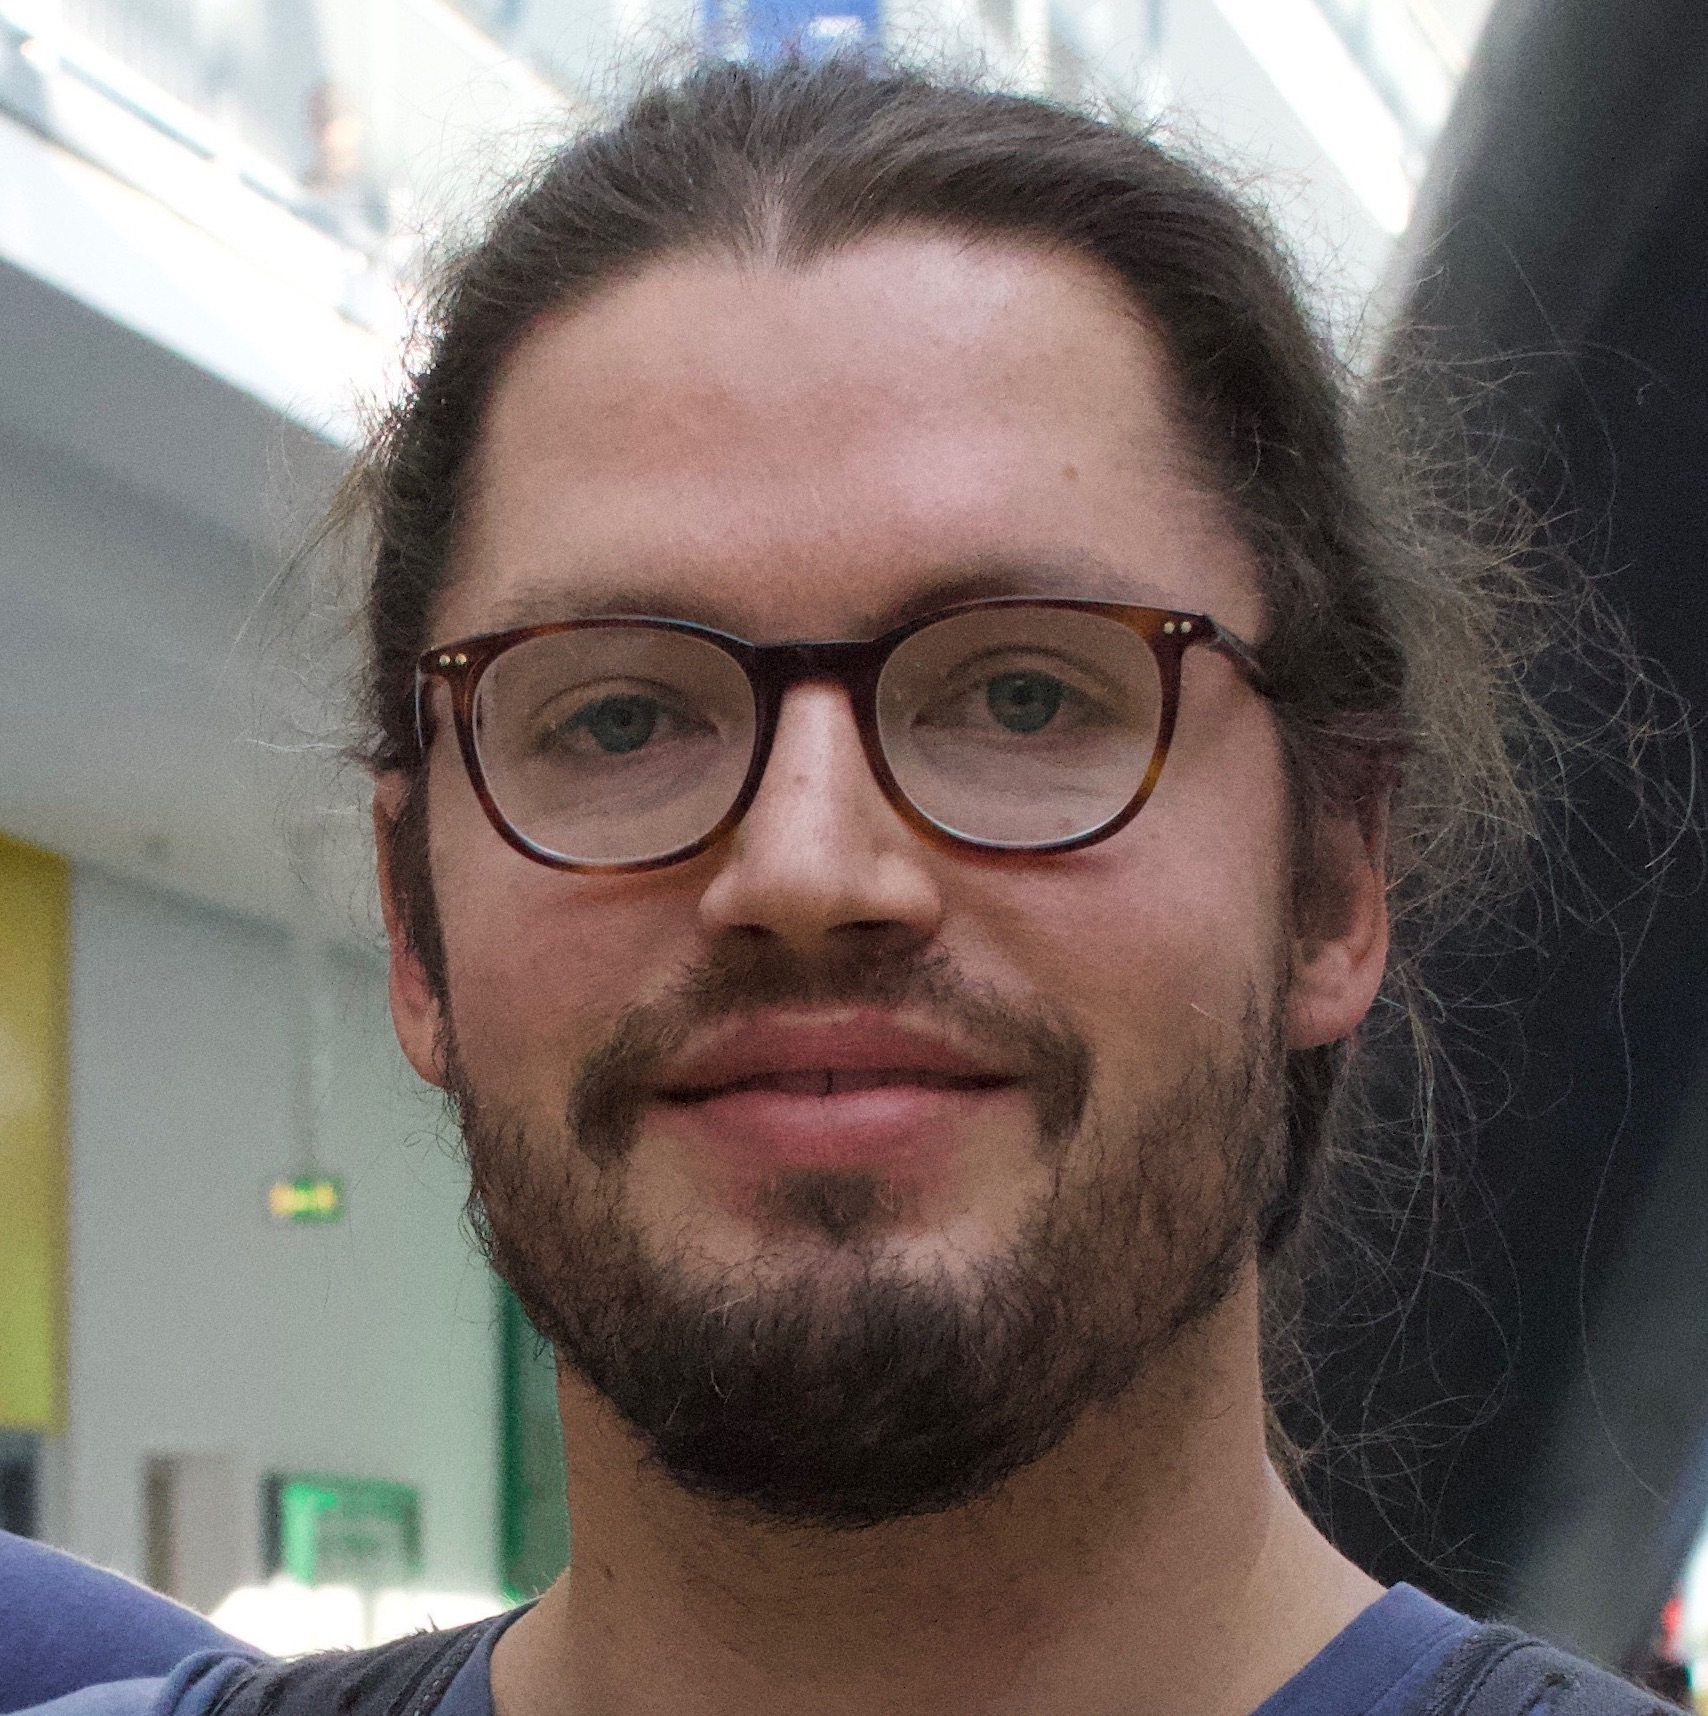
\includegraphics[height=1.5cm,width=1.5cm]{0-fig-people/jf2.jpg} \hspace{7em}%
  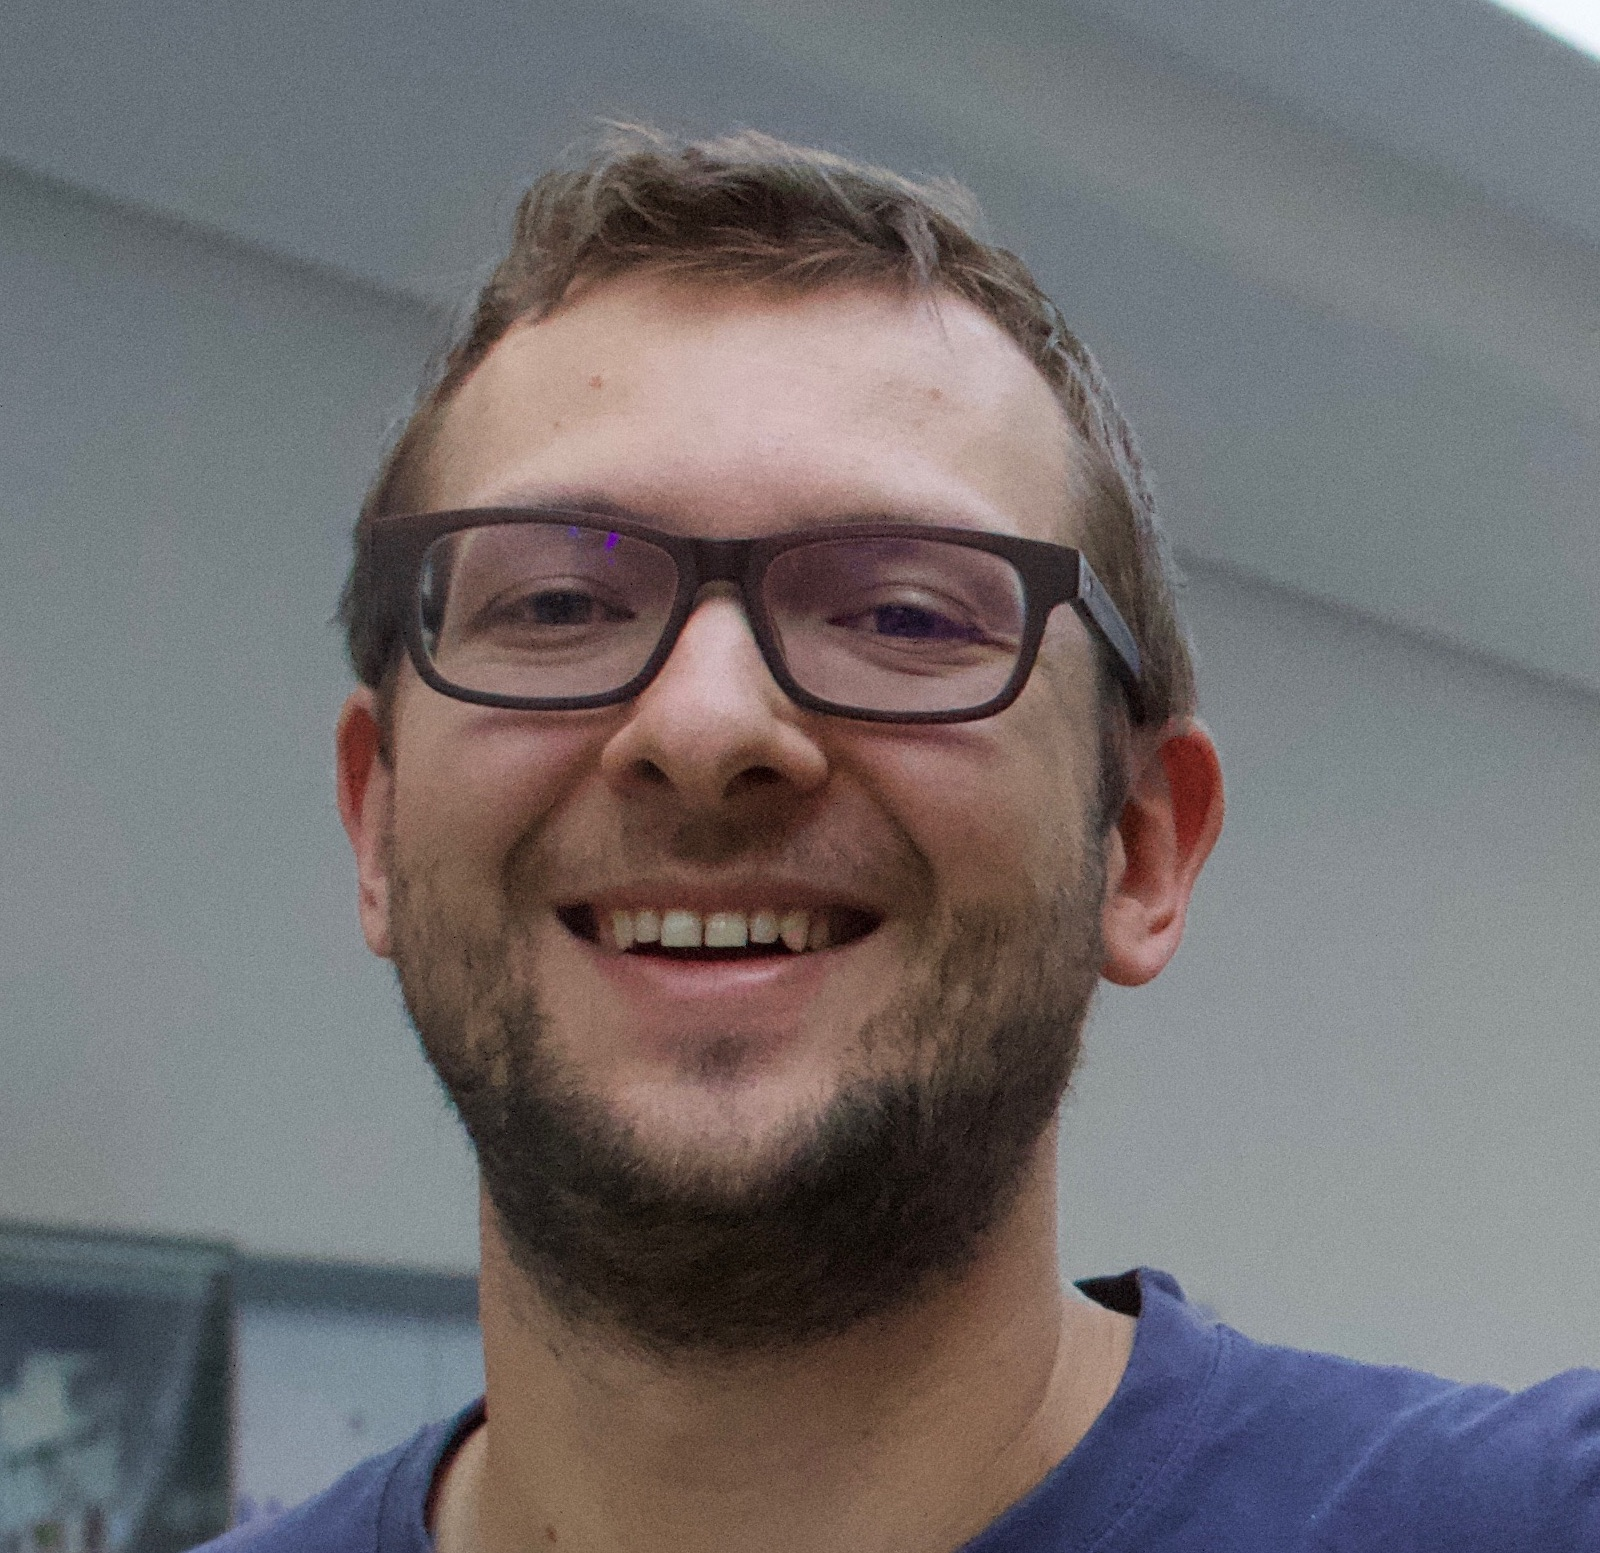
\includegraphics[height=1.5cm,width=1.5cm]{0-fig-people/mh2.jpg} \hspace{7em}%
  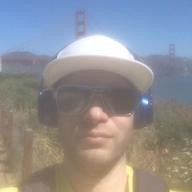
\includegraphics[height=1.5cm,width=1.5cm]{0-fig-people/pt.jpg} \hspace{7em}%
  
\includegraphics[height=1.5cm,width=1.7cm]{0-fig-people/sw2.jpg} \hspace{7em}%
  \\
  \vspace{0.5em}
  22nd International Symposium on Practical Aspects\\
  of Declarative Languages (PADL 2020)\\[1em]
  New Orleans, LA, USA January 21, 2020%
}%
\institute{%
  $^1$TU Dresden, Germany\\[0.5ex]
  $^2$TU Wien, Austria\\[0.5ex]
  \tiny{$^3${University of Potsdam, Germany}}\\[2em]
  % Grants Y698, W1255-N23, P-26696\\[2.5em]%
  % %\tiny{$^3${Johannes Kepler University Linz, Austria}}%
  % %\\[2.5em]%\\[-0.2em]%
  % 
}

\usepackage{mytikz}
\newcommand{\pgftextsize}{\scriptsize}

\newcommand{\unchecked}{{\Large\makebox[0pt][l]{\phantom{$\square$}}\raisebox{.15ex}{\hspace{0.1em}}}}
\newcommand{\checked}{{\Large\makebox[0pt][l]{\phantom{$\square$}}\raisebox{.1ex}{\hspace{0.1em}$\checkmark$}}}

\usepackage{hanging}
\begin{document}
\loadpresentation{0-figs/graph0/td1.tex}
\loadpresentation{0-figs/graph0/td2.tex}



\section{Introduction}


\setcounter{framenumber}{0}
\maketitle


\begin{frame}{Motivation}
  \vspace{-1em}
  \begin{block}{Domain}
    \begin{itemize}
    \item Hard problems tractable when certain properties present
    \item Examples: Vertex Cover, Model Counting (\#SAT), ...
    \item \alert{Bounded treewidth} often leads to tractability in theory,
      e.g., problems expressible in monadic second-order logic (MSO)
    \end{itemize}
  \end{block}
  \vspace{-1em}
  \begin{block}{Approaches \uncover<2>{({\color{blue}Advantages}/{\color{red}Disadvantages})}:}
    \begin{enumerate}
    \item Design dynamic programming algorithm (DP) and implement it
    \item[\hspace{2em}\cmark]<2-> {\color{blue}Can perform well (e.g., gpusat \bcite{FHWZisser'18})}
    \item[\hspace{2em}\xmark\hspace{0.25em}]<2-> {\color{red}Pretty annoying to implement}
    \item Use MSO solver together with an MSO specification 
    \item[\hspace{2em}\xmark\hspace{0.25em}]<2-> {\color{red}Does not perform (e.g., Sequoia \bcite{Kneis\&Langer\&Rossmanith'11})}
    \item[\hspace{2em}\cmark]<2-> {\color{blue}Easy to implement and many theoretical descriptions available}
    \end{enumerate}
  \end{block}
\end{frame}


\begin{frame}{Research Question \uncover<2>{\& Approach}}
  \medskip
  \alert{Can we merge the two approaches? (and make it reasonable to use?)}\\[0.5em]
  \begin{itemize}
  \item[Idea 1:] Provide a programming framework.\\
    Already done.\\
    $\Rightarrow$ Sharp (C++) \bcite{Morak'11} and Jatatosk (Java) \bcite{Bannach\&Berndt'18}\\
    \hspace{1em}\xmark~still hard to use \hspace{4.7em} \xmark~performs nice, but far from competitive
    \medskip
  \item[Idea 2:] Use a logic based language to specify the DP\\
    Already done.\\
    $\Rightarrow$ D-FLAT (use ASP for spec and take an ASP solver for
    computation) \bcite{Bliem\&Morak\&Stefan Woltran'12}\\
    \hspace{1em}\xmark~still fairly hard to use and performs mostly not very well
    \color{red}
  \end{itemize}
  \uncover<2->{%
    
    \color{red}Our idea Use SQL to describe the DP and use a DBMS to
    evaluate the queries
    
  }
\end{frame}

\begin{frame}{Outline}
\bigskip\bigskip\bigskip
  \begin{enumerate}
  \item Basics: Tree Decompositions\medskip
  \item Dynamic Programming Example and Computation for Model Counting
    (\#SAT)\medskip
  \item Our tool \texttt{dpdb}
  \end{enumerate}
\end{frame}

\subsection{Preliminaries}
\begin{frame}<1,2,10>[noframenumbering]{Tree Decompositions}\label{lbl:motivation}
  \only<1>{
  \bigskip
  \begin{columns}
    \begin{column}{0.5\textwidth}
      {\includegraphics[scale=0.15]{0-figs/tw}}
    \end{column}
    \begin{column}{0.5\textwidth}
      \includegraphics[scale=0.18]{0-figs/treedecomp}
    \end{column}
  \end{columns}    
  }%
  \only<2->{%
    \begin{center}
      \vspace{-2em}
      \begin{columns}
        \begin{column}{0.3\textwidth}
          \input{0-figs/graph0/graph2_m}
        \end{column}
        \begin{column}{0.3\textwidth}
          \uncover<10->{%
            \input{0-figs/graph0/td}
            %
          }%
        \end{column}
      \end{columns}
      \vspace{-3em}
    \end{center}
    % 
  }%

  \only<1>{%

  \begin{block}{Treewidth \hyperlink{treewidth}{\beamergotobutton{Definition \& Example}}}
    %\vspace{-0.5em}
    \begin{itemize}\itemsep5pt
    \item<1> Most prominent graph invariant 
    \item<1> Small treewidth indicates tree-likeness and sparsity
    \item<1> Can be used to solve \#SAT/WMC by defining graph\\
      representations of the input formula
    \end{itemize}
  \end{block}
  }%
  \only<2,10>{%
    \begin{block}{Treewidth \hyperlink{treewidth}{\beamergotobutton{Definition \& Example}}}
      % \vspace{-0.5em}
      \begin{itemize}\itemsep5pt
      \item Treewidth defined in terms of tree decompositions (TD)
      \item TD: arrangement of graph into a tree of bags s.t. ...
      \item<10> Treewidth: width of a TD of smallest width
      \end{itemize}
    \end{block}
  }%
\end{frame}

% \section{Tree Decompositions}
% \begin{frame}{``Treewidth''?}
%   \begin{columns}
%     \column{.05\textwidth}
%     \column{.65\textwidth}
%     {\includegraphics[scale=0.2]{0-figs/tw.jpg}}
%   \end{columns}
%   \begin{itemize}
%     \medskip
%   \item Many problems are (comput.) hard on graphs, but simpler on trees
%     \medskip
%   \item There is a way to capture how \alert{``tree-like''} a graph is -- the
%     treewidth, defined in terms of
%     \alert{tree decompositions} $\dots$
%     % 
%   \end{itemize}
% \end{frame}


%,label=td
\begin{frame}<10>[label=td]{Tree Decompositions}
  \begin{columns}[T]
    \begin{column}{.463\textwidth}
      \includegraphics[scale=0.21]{0-figs/treedecomp.jpg}
    \end{column}
    \begin{column}{.48\textwidth}
      \vspace{-1em}
      \begin{exampleblock}{Tree Decomposition $\mathcal{T}$ of $G$}
        \vspace{-1em}
        \begin{columns}
          \begin{column}{0.5\textwidth}
            \centering ~\hspace{1em}\input{0-figs/graph0/graph2_m}
          \end{column}
          \begin{column}{0.5\textwidth}
            \input{0-figs/graph0/td}\\[1em]
          \end{column}
        \end{columns}
      \end{exampleblock}
    \end{column}
  \end{columns}
  \vspace{-2.5ex}
  \begin{block}{Definition}
    % \hyperlink{tw_basics<1>}{\beamergotobutton{Formally}}}
    A tree decomposition is a tree obtained from an arbitrary graph
    s.t.\
    \begin{enumerate}
    \item \textcolor<2>{red}{Each vertex} must occur in some
      \emph{bag}
    \item For \textcolor<3-7>{red}{each edge}, there is a bag
      containing both endpoints
    \item %\emph{Connectedness condition}:\\
      \textcolor<8-9>{red}{\emph{Connected}}: Tree ``restricted'' to any vertex must be connected
    \end{enumerate}
  \end{block}
\end{frame}




\begin{frame}[noframenumbering]{}
  \bigskip
  \bigskip
  \bigskip
  \bigskip
  \bigskip
  \bigskip
  \begin{center}
    \alert{\Large ``Find'' tree decompositions of small width?}\\

    \bigskip

    \uncover<2>{%
      Works well even for relatively large instances.\\[1em]
      Thanks to the Parameterized Algorithms and\\
      Computational Experiments Challenge \\
      (PACE) '16/'17!!!
      %
    }

  \end{center}
\end{frame}


\begin{frame}[noframenumbering]{}
  \bigskip
  \bigskip
  \bigskip
  \bigskip
  \bigskip
  \bigskip
  \begin{center}
    \alert{\Large How to ``use'' tree decompositions for \#SAT/WMC?}\\
  \end{center}
\end{frame}

\begin{frame}{Approach / Dynamic Programming}
  \bigskip\bigskip\bigskip
  \centering
  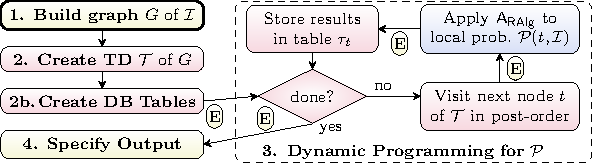
\includegraphics[scale=1.2]{0-figs/figure}
\end{frame}


\begin{frame}<1-5,11,16>[label=sat]{Example Problem of Interest}
  \medskip
  \begin{block}{SAT-Problem (Boolean Satisfiability Problem)}
    \begin{tabular}[t]{ll}
      Given: & Propositional formula $F$.\\
      Question: & Is there a truth assignment~$\tau$ to the variables\\
             & in $F$ such that $F_\tau$ evaluates to $1$ (\emph{satisfiable}).
    \end{tabular}\\
    %\hfill\hyperlink{sat<16>}{\beamergotobutton{Skip Example}}
  \end{block}
  \vspace{-1.2em}
  \only<1-2>{
  \uncover<2->{
  \begin{block}{Input normal form}
    \begin{itemize}
    \item Conjunctive normal form (CNF)
    \item Form:
      $F = (\ell_1 \vee \ell_2 \vee \ell_3) \wedge \ldots \wedge
      (\ldots)$
 where $\ell_i$ either $x$ or $\neg x$
    \end{itemize}
  \end{block}
  }}
  \only<3->{
    \begin{block}{Example}
      % -1 -2 3 4 5 0
      \only<1-20>{%
        \vspace{-2em}
        \only<3>{%
          \vspace{0.5em}
          \begin{align*}
            F = ( \neg a \vee b \vee x) \wedge (a \vee b) \wedge (c \vee \neg x) \wedge (b \vee \neg c) \wedge (\neg b \vee \neg c \vee \neg y)
          \end{align*}
        } %
        \only<4>{%
          \begin{align*}
            F = ( \neg \vf{a} \vee \vt{b} \vee \vf{x}) \wedge 
            (\vf{a} \vee \vt{b}) \wedge (\vf{c} \vee \neg \vf{x}) 
            \wedge (\vt{b} \vee \neg \vf{c}) \wedge 
            (\neg \vt{b} \vee \neg \vf{c} \vee \neg \vf{y})
          \end{align*}
        }
        \only<5->{%
          \begin{align*}
            F = \cancelto{1}{( \neg \vf{a} \vee \vt{b} \vee \vf{x})} \wedge 
            \cancelto{1}{(\vf{a} \vee \vt{b})} \wedge 
            \cancelto{1}{(\vf{c} \vee \neg \vf{x})} 
            \cancelto{1}{\wedge (\vt{b} \vee \neg \vf{c})} \wedge 
            \cancelto{1}{(\neg \vt{b} \vee \neg \vf{c} \vee \neg \vf{y})}
          \end{align*}
        }
        \\[0.5em]
        \only<11->{%
          \begin{center}
            \alert{%
              $\Rightarrow$ Satisfiable\\[1em]
            }
          \end{center}
        }%  
      }%
    \end{block}
  }
  \uncover<16->{%
    \begin{block}{Model Counting (\#SAT/Number SAT)}
      \begin{itemize}
      \item Number of of satisfying truth assignments to~$F$.
      \end{itemize}
    \end{block}
    %
  }%
\end{frame}



\newcommand{\hsep}{\ensuremath{\leftarrow}}
\begin{frame}<-2>[label=solving]{Solving \#SAT \textcolor{blue}{[SamerSzeider10]}}
  \vspace{-0.5em}
  \begin{exampleblock}{$F=$\textcolor<4>{red}{$(\neg a \vee b
        \vee x)$} $\wedge$ \textcolor<4>{red}{$(a \vee b)$} $\wedge$
      \textcolor<5>{red}{$(c \vee \neg x)$} $\wedge$
      \textcolor<5-9>{red}{$(b \vee \neg c)$} $\wedge$
      \textcolor<7>{red}{$(\neg b \vee \neg c \vee \neg y)$}}
    \only<1>{
      \vspace{-1.5em}
      \begin{align*}
        \mathit{Mod}(F) & =\{ &
                                      \{b\},
                                      \{a,b\},
                                      \{b,c\}, 
                                      \{a,b,c\}, \\
                              &&
                                 \{b,c,x\},
                                 \{a,b,c,x\},\\
                              &&
                                 \{b,y\},
                                 \{a,b,y\}
                                 \}
      \end{align*}
      \vspace{-4em}
    }%
    %\uncover<3->{\include{0-figs/graphplus/graph_m_simple}}
    \begin{columns}[T]
      \begin{column}{.5\textwidth}
        %\vspace{-1em}
        \begin{enumerate}
        \item<2-> Create graph representation
        \item<3-> Decompose graph
        \item<4-> Solve subproblems
        \item<11-> Combine rows
      \end{enumerate}
      \uncover<3->{%
        \vspace{-1em}
        \begin{tikzpicture}[font=\small,baseline={(current bounding box.south)}]%
          \tikzset{ every node/.style={anchor=north} }%
          \node[] at (5.5,3.65) (nid) {};%
          \node[tdnode, label=right:{$ $}] at (5.5,2.9) (n8)
          {$b,\; c$};%
          \node <9> [color=red,tdnode,
          label=right:\textcolor{red}{$ $}] at (5.5,2.9) (n8)
          {$b,\; c$};%
          \node[tdnode, label=left:{$ $}] at (4.7,2.2) (n4)
          {$b,\; c$};%
          \node <6> [color=red,tdnode,
          label=left:\textcolor{red}{$ $}] at (4.7,2.2) (n4)
          {$b,\; \textcolor{red}{c}\textcolor{red}{}$};%
          \node [tdnode, label=left:{$ $}] at (4.7,1.5) (n10)
          {$b,\;x,\;c$};%
          \node <5> [color=red, tdnode,
          label=left:\textcolor{red}{$ $}] at (4.7,1.5) (n10)
          {$b,\;x,\;c$};%
          \node [tdnode, label={[xshift=0.4cm]left:{$\qquad\quad $}}]
          at (4.7,0.8) (n1) {$b,\; x,\; a$};%
          \node <4> [color=red, tdnode,
          label={[xshift=0.4cm]left:\textcolor{red}{$\qquad\quad $}}]
          at (4.7,0.8) (n1)
          {$\textcolor{red}{b,\; x,\; a}\textcolor{red}{}$};%
 
          \node[tdnode, label=above right:{$ $}] at (6.5,2.2) (n7)
          {$b,\; c$};%
          \node <8> [color=red,tdnode, label=above
          right:\textcolor{red}{$ $}] at (6.5,2.2) (n7) {$b,\; c$};%
          \node <8> [color=red,tdnode, label=above
          right:\textcolor{red}{$ $}] at (6.5,2.2) (n7)
          {$\textcolor{red}{b,\; c}$};%
          \node[tdnode, label=left:{$ $}] at (6.5,1.5) (n6)
          {$b,\;c,\;y$};%
          \node <7> [color=red,tdnode,
          label=left:\textcolor{red}{$ $}] at (6.5,1.5) (n6)
          {$b,\;c,\;y$};%
          \draw[tdedge] (n8) -- (n4) -- (n10) -- (n1);%
          \draw[tdedge] (n8) -- (n7) -- (n6);%
        \end{tikzpicture}%
      }%
      \\
      \vspace{1em}%
      \hspace{1em} \only<4->{%
        ``Local formula''~$F_t$ clauses whose\\ \hspace{1.2em} variables are
        contained in the bag\\ \hspace{1.5em}\uncover<4->{(colored in red above)}
        % 
      }
    \end{column}
    \begin{column}{.5\textwidth}
      \medskip
      \only<2>{%
        \vspace{2em}
        \resizebox{0.5\columnwidth}{!}{%
          {\color{blue}
        \begin{tikzpicture}[font=\small,baseline={(current bounding box.center)}]%
          \tikzset{ every node/.style={anchor=north} }%
          \node[](a){a};
          \node[left of=a](b){b};
          \node[below of=a](x){x};

          \node[left of=x](c){c};
          \node[left of=c](y){y};

          \draw[] (a) -- (b) -- (x) -- (a);%
          \draw[] (c) -- (x); %
          \draw[] (b) -- (c) -- (y) -- (b);%
        \end{tikzpicture}%        
        }%
        %
        }%
      }%
      \only<3>{%
        {~ %Determine origin row, copy values for current-bag and handle
        \begin{itemize}
        \item[LEAF.:] Put empty set and counter 1
        \item[INTR.:]
          Guess truth value and check satisfiability 
          %\begin{itemize} 
% ($a \mapsto 0$ or $a \mapsto 1$)
%           \item Consider $\tau_a = \tau \cup \{a \mapsto 1\}$ and
%             $\tau_{\neg a} = \tau \cup \{a \mapsto 0\}$\\
%             (old assignment with(out) a)
%           \item Check satisfiability\\
%             ($\tau_a \models F_t$? $\tau_{\neg a} \models F_t$?)
          %\end{itemize}
          % \item[INTR. clause:] Mark if satisfied
        \item[REMOVE:] Remove $a$ from each assignment (row) in the
          table and sum up the counters if we get multiple assignments
          with the same data
        %\item[REM. clause:] Check satisfiability
        \item[JOIN:] Match rows with the same assignment and multiply
          the counters
        %\item[JOIN clause:] Mark if satisfied in some origin row
        \end{itemize} 
        % \begin{itemize}
        % \item[INTR. atom:] Guess truth-value, mark sat. clauses
        % \item[INTR. clause:] Mark if satisfied
        % \item[REMOVE atom:] Nothing to do
        % \item[REM. clause:] Check satisfiability
        % \item[JOIN atom:] Check truth-value agreement
        % \item[JOIN clause:] Mark if satisfied in some origin row
        % \end{itemize} 
        }
        % 
      }
      \only<4-11>{\def\highlightthings{\rowcolor<11> {HighlightColor}}
        \input{0-figs/graph0/ids-tables/tables_sat}}%
      \only<12->{\def\highlightthings{ }
        \input{0-figs/graph0/ids-tables/tables_ssat}}
      \vspace{1ex}
    \end{column}
  \end{columns}
  \end{exampleblock}
\end{frame}


%\section{Answer Set Programming}
%\newcommand{\hsep}{\ensuremath{\leftarrow}}
\begin{frame}<3->[]{Solving \#SAT \textcolor{blue}{[SamerSzeider'10]}}
  \vspace{-0.5em}
  \begin{exampleblock}{$F=$\textcolor<4>{red}{$(\neg a \vee b
        \vee x)$} $\wedge$ \textcolor<4>{red}{$(a \vee b)$} $\wedge$
      \textcolor<5>{red}{$(c \vee \neg x)$} $\wedge$
      \textcolor<5-9>{red}{$(b \vee \neg c)$} $\wedge$
      \textcolor<7>{red}{$(\neg b \vee \neg c \vee \neg y)$}}
    \only<1>{
      \vspace{-1.5em}
      \begin{align*}
        \mathit{Mod}(F) & =\{ &
                                      \{b\},
                                      \{a,b\},
                                      \{b,c\}, 
                                      \{a,b,c\}, \\
                              &&
                                 \{b,c,x\},
                                 \{a,b,c,x\},\\
                              &&
                                 \{b,y\},
                                 \{a,b,y\}
                                 \}
      \end{align*}
      \vspace{-4em}
    }%
    %\uncover<3->{\include{0-figs/graphplus/graph_m_simple}}
    \begin{columns}[T]
      \begin{column}{.5\textwidth}
        %\vspace{-1em}
        \begin{enumerate}
        \item<2-> Create graph representation
        \item<3-> Decompose graph
        \item<4-> Solve subproblems
        \item<11-> Combine rows
      \end{enumerate}
      \uncover<3->{%
        \vspace{-1em}
        \begin{tikzpicture}[font=\small,baseline={(current bounding box.south)}]%
          \tikzset{ every node/.style={anchor=north} }%
          \node[] at (5.5,3.65) (nid) {};%
          \node[tdnode, label=right:{$ $}] at (5.5,2.9) (n8)
          {$b,\; c$};%
          \node <9> [color=red,tdnode,
          label=right:\textcolor{red}{$ $}] at (5.5,2.9) (n8)
          {$b,\; c$};%
          \node[tdnode, label=left:{$ $}] at (4.7,2.2) (n4)
          {$b,\; c$};%
          \node <6> [color=red,tdnode,
          label=left:\textcolor{red}{$ $}] at (4.7,2.2) (n4)
          {$b,\; \textcolor{red}{c}\textcolor{red}{}$};%
          \node [tdnode, label=left:{$ $}] at (4.7,1.5) (n10)
          {$b,\;x,\;c$};%
          \node <5> [color=red, tdnode,
          label=left:\textcolor{red}{$ $}] at (4.7,1.5) (n10)
          {$b,\;x,\;c$};%
          \node [tdnode, label={[xshift=0.4cm]left:{$\qquad\quad $}}]
          at (4.7,0.8) (n1) {$b,\; x,\; a$};%
          \node <4> [color=red, tdnode,
          label={[xshift=0.4cm]left:\textcolor{red}{$\qquad\quad $}}]
          at (4.7,0.8) (n1)
          {$\textcolor{red}{b,\; x,\; a}\textcolor{red}{}$};%
 
          \node[tdnode, label=above right:{$ $}] at (6.5,2.2) (n7)
          {$b,\; c$};%
          \node <8> [color=red,tdnode, label=above
          right:\textcolor{red}{$ $}] at (6.5,2.2) (n7) {$b,\; c$};%
          \node <8> [color=red,tdnode, label=above
          right:\textcolor{red}{$ $}] at (6.5,2.2) (n7)
          {$\textcolor{red}{b,\; c}$};%
          \node[tdnode, label=left:{$ $}] at (6.5,1.5) (n6)
          {$b,\;c,\;y$};%
          \node <7> [color=red,tdnode,
          label=left:\textcolor{red}{$ $}] at (6.5,1.5) (n6)
          {$b,\;c,\;y$};%
          \draw[tdedge] (n8) -- (n4) -- (n10) -- (n1);%
          \draw[tdedge] (n8) -- (n7) -- (n6);%
        \end{tikzpicture}%
      }%
      \\
      \vspace{1em}%
      \hspace{1em} \only<4>{%
        ``Local formula''~$F_t$ clauses whose\\ \hspace{1.2em} variables are
        contained in the bag\\ \hspace{1.5em}\uncover<4>{(colored in red above)}
        % 
      }
    \end{column}
    \begin{column}{.5\textwidth}
      \medskip
      \only<2>{%
        \vspace{2em}
        \resizebox{0.5\columnwidth}{!}{%
          {\color{blue}
        \begin{tikzpicture}[font=\small,baseline={(current bounding box.center)}]%
          \tikzset{ every node/.style={anchor=north} }%
          \node[](a){a};
          \node[left of=a](b){b};
          \node[below of=a](x){x};

          \node[left of=x](c){c};
          \node[left of=c](y){y};

          \draw[] (a) -- (b) -- (x) -- (a);%
          \draw[] (c) -- (x); %
          \draw[] (b) -- (c) -- (y) -- (b);%
        \end{tikzpicture}%        
        }%
        %
        }%
      }%
      \only<4-11>{\def\highlightthings{\rowcolor<11> {HighlightColor}}
        \input{0-figs/graph0/ids-tables/tables_sat}}%
      \only<12->{\def\highlightthings{ }
        \input{0-figs/graph0/ids-tables/tables_ssat}}
      \vspace{1ex}
    \end{column}
  \end{columns}
  \end{exampleblock}
\end{frame}


% \begin{frame}<3>[label=current]{Solving \#SAT \textcolor{blue}{[SamerSzeider'10]}}
%   \vspace{-0.5em}
%   \begin{exampleblock}{$F=$\textcolor<4>{red}{$(\neg a \vee b
%         \vee x)$} $\wedge$ \textcolor<4>{red}{$(a \vee b)$} $\wedge$
%       \textcolor<5>{red}{$(c \vee \neg x)$} $\wedge$
%       \textcolor<5-9>{red}{$(b \vee \neg c)$} $\wedge$
%       \textcolor<7>{red}{$(\neg b \vee \neg c \vee \neg y)$}}
%     \only<1>{
%       \vspace{-1.5em}
%       \begin{align*}
%         \mathit{Mod}(F) & =\{ &
%                                       \{b\},
%                                       \{a,b\},
%                                       \{b,c\}, 
%                                       \{a,b,c\}, \\
%                               &&
%                                  \{b,c,x\},
%                                  \{a,b,c,x\},\\
%                               &&
%                                  \{b,y\},
%                                  \{a,b,y\}
%                                  \}
%       \end{align*}
%       \vspace{-4em}
%     }%
%     %\uncover<3->{\include{0-figs/graphplus/graph_m_simple}}
%     \begin{columns}[T]
%       \begin{column}{.5\textwidth}
%         %\vspace{-1em}
%         \begin{enumerate}
%         \item<2-> Create graph representation
%         \item<3-> Decompose graph
%         \item<4-> Solve subproblems
%         \item<11-> Combine rows
%       \end{enumerate}
%       \uncover<3->{%
%         \vspace{-1em}
%         \begin{tikzpicture}[font=\small,baseline={(current bounding box.south)}]%
%           \tikzset{ every node/.style={anchor=north} }%
%           \node[] at (5.5,3.65) (nid) {};%
%           \node[tdnode, label=right:{$ $}] at (5.5,2.9) (n8)
%           {$b,\; c$};%
%           \node <9> [color=red,tdnode,
%           label=right:\textcolor{red}{$ $}] at (5.5,2.9) (n8)
%           {$b,\; c$};%
%           \node[tdnode, label=left:{$ $}] at (4.7,2.2) (n4)
%           {$b,\; c$};%
%           \node <6> [color=red,tdnode,
%           label=left:\textcolor{red}{$ $}] at (4.7,2.2) (n4)
%           {$b,\; \textcolor{red}{c}\textcolor{red}{}$};%
%           \node [tdnode, label=left:{$ $}] at (4.7,1.5) (n10)
%           {$b,\;x,\;c$};%
%           \node <5> [color=red, tdnode,
%           label=left:\textcolor{red}{$ $}] at (4.7,1.5) (n10)
%           {$b,\;x,\;c$};%
%           \node [tdnode, label={[xshift=0.4cm]left:{$\qquad\quad $}}]
%           at (4.7,0.8) (n1) {$b,\; x,\; a$};%
%           \node <4> [color=red, tdnode,
%           label={[xshift=0.4cm]left:\textcolor{red}{$\qquad\quad $}}]
%           at (4.7,0.8) (n1)
%           {$\textcolor{red}{b,\; x,\; a}\textcolor{red}{}$};%
 
%           \node[tdnode, label=above right:{$ $}] at (6.5,2.2) (n7)
%           {$b,\; c$};%
%           \node <8> [color=red,tdnode, label=above
%           right:\textcolor{red}{$ $}] at (6.5,2.2) (n7) {$b,\; c$};%
%           \node <8> [color=red,tdnode, label=above
%           right:\textcolor{red}{$ $}] at (6.5,2.2) (n7)
%           {$\textcolor{red}{b,\; c}$};%
%           \node[tdnode, label=left:{$ $}] at (6.5,1.5) (n6)
%           {$b,\;c,\;y$};%
%           \node <7> [color=red,tdnode,
%           label=left:\textcolor{red}{$ $}] at (6.5,1.5) (n6)
%           {$b,\;c,\;y$};%
%           \draw[tdedge] (n8) -- (n4) -- (n10) -- (n1);%
%           \draw[tdedge] (n8) -- (n7) -- (n6);%
%         \end{tikzpicture}%
%       }%
%       \\
%       \vspace{1em}%
%       \hspace{1em} \only<2->{%
%         ``Local formula''~$F_t$ clauses whose\\ \hspace{1.2em} variables are
%         contained in the bag\\ \hspace{1.5em}\uncover<3->{(colored in red above)}
%         % 
%       }
%     \end{column}
%     \begin{column}{.5\textwidth}
%       \medskip
%       \only<2>{%
%         \vspace{2em}
%         \resizebox{0.5\columnwidth}{!}{%
%           {\color{blue}
%         \begin{tikzpicture}[font=\small,baseline={(current bounding box.center)}]%
%           \tikzset{ every node/.style={anchor=north} }%
%           \node[](a){a};
%           \node[left of=a](b){b};
%           \node[below of=a](x){x};

%           \node[left of=x](c){c};
%           \node[left of=c](y){y};

%           \draw[] (a) -- (b) -- (x) -- (a);%
%           \draw[] (c) -- (x); %
%           \draw[] (b) -- (c) -- (y) -- (b);%
%         \end{tikzpicture}%        
%         }%
%         %
%         }%
%       }%
%       \only<3>{%
%         {~ %Determine origin row, copy values for current-bag and handle
%           Nice Tree Decompositions\\
%           (note example left is not nice)
%           \begin{itemize}
%           \item[LEAF.:] Put empty set and counter 1
%           \item[INTR.:]
%             Guess truth value and check satisfiability 
%           %\begin{itemize} 
% % ($a \mapsto 0$ or $a \mapsto 1$)
% %           \item Consider $\tau_a = \tau \cup \{a \mapsto 1\}$ and
% %             $\tau_{\neg a} = \tau \cup \{a \mapsto 0\}$\\
% %             (old assignment with(out) a)
% %           \item Check satisfiability\\
% %             ($\tau_a \models F_t$? $\tau_{\neg a} \models F_t$?)
%           %\end{itemize}
%           % \item[INTR. clause:] Mark if satisfied
%         \item[REMOVE:] Remove $a$ from each assignment (row) in the
%           table and sum up the counters if we get multiple assignments
%           with the same data
%         %\item[REM. clause:] Check satisfiability
%         \item[JOIN:] Match rows with the same assignment and multiply
%           the counters
%         %\item[JOIN clause:] Mark if satisfied in some origin row
%         \end{itemize} 
%         % \begin{itemize}
%         % \item[INTR. atom:] Guess truth-value, mark sat. clauses
%         % \item[INTR. clause:] Mark if satisfied
%         % \item[REMOVE atom:] Nothing to do
%         % \item[REM. clause:] Check satisfiability
%         % \item[JOIN atom:] Check truth-value agreement
%         % \item[JOIN clause:] Mark if satisfied in some origin row
%         % \end{itemize} 
%         }
%         % 
%       }
%       \only<4-11>{\def\highlightthings{\rowcolor<11> {HighlightColor}}
%         \input{0-figs/graph0/ids-tables/tables_sat}}%
%       \only<12->{\def\highlightthings{ }
%         \input{0-figs/graph0/ids-tables/tables_ssat}}
%       \vspace{1ex}
%     \end{column}
%   \end{columns}
%   \end{exampleblock}
% \end{frame}

\begin{frame}<3>[label=current]{Solving \#SAT \textcolor{blue}{[SamerSzeider'10]}}
  \vspace{-0.5em}
  \begin{exampleblock}{$F=$\textcolor<4>{red}{$(\neg a \vee b
        \vee x)$} $\wedge$ \textcolor<4>{red}{$(a \vee b)$} $\wedge$
      \textcolor<5>{red}{$(c \vee \neg x)$} $\wedge$
      \textcolor<5-9>{red}{$(b \vee \neg c)$} $\wedge$
      \textcolor<7>{red}{$(\neg b \vee \neg c \vee \neg y)$}}
    \only<1>{
      \vspace{-1.5em}
      \begin{align*}
        \mathit{Mod}(F) & =\{ &
                                      \{b\},
                                      \{a,b\},
                                      \{b,c\}, 
                                      \{a,b,c\}, \\
                              &&
                                 \{b,c,x\},
                                 \{a,b,c,x\},\\
                              &&
                                 \{b,y\},
                                 \{a,b,y\}
                                 \}
      \end{align*}
      \vspace{-4em}
    }%
    %\uncover<3->{\include{0-figs/graphplus/graph_m_simple}}
    \begin{columns}[T]
      \begin{column}{.5\textwidth}
        %\vspace{-1em}
        \begin{enumerate}
        \item<2-> Create graph representation
        \item<3-> Decompose graph
        \item<4-> Solve subproblems
        \item<11-> Combine rows
      \end{enumerate}
      \uncover<3->{%
        \vspace{-1em}
        \begin{tikzpicture}[font=\small,baseline={(current bounding box.south)}]%
          \tikzset{ every node/.style={anchor=north} }%
          \node[] at (5.5,3.65) (nid) {};%
          \node[tdnode, label=right:{$ $}] at (5.5,2.9) (n8)
          {$b,\; c$};%
          \node <9> [color=red,tdnode,
          label=right:\textcolor{red}{$ $}] at (5.5,2.9) (n8)
          {$b,\; c$};%
          \node[tdnode, label=left:{$ $}] at (4.7,2.2) (n4)
          {$b,\; c$};%
          \node <6> [color=red,tdnode,
          label=left:\textcolor{red}{$ $}] at (4.7,2.2) (n4)
          {$b,\; \textcolor{red}{c}\textcolor{red}{}$};%
          \node [tdnode, label=left:{$ $}] at (4.7,1.5) (n10)
          {$b,\;x,\;c$};%
          \node <5> [color=red, tdnode,
          label=left:\textcolor{red}{$ $}] at (4.7,1.5) (n10)
          {$b,\;x,\;c$};%
          \node [tdnode, label={[xshift=0.4cm]left:{$\qquad\quad $}}]
          at (4.7,0.8) (n1) {$b,\; x,\; a$};%
          \node <4> [color=red, tdnode,
          label={[xshift=0.4cm]left:\textcolor{red}{$\qquad\quad $}}]
          at (4.7,0.8) (n1)
          {$\textcolor{red}{b,\; x,\; a}\textcolor{red}{}$};%
 
          \node[tdnode, label=above right:{$ $}] at (6.5,2.2) (n7)
          {$b,\; c$};%
          \node <8> [color=red,tdnode, label=above
          right:\textcolor{red}{$ $}] at (6.5,2.2) (n7) {$b,\; c$};%
          \node <8> [color=red,tdnode, label=above
          right:\textcolor{red}{$ $}] at (6.5,2.2) (n7)
          {$\textcolor{red}{b,\; c}$};%
          \node[tdnode, label=left:{$ $}] at (6.5,1.5) (n6)
          {$b,\;c,\;y$};%
          \node <7> [color=red,tdnode,
          label=left:\textcolor{red}{$ $}] at (6.5,1.5) (n6)
          {$b,\;c,\;y$};%
          \draw[tdedge] (n8) -- (n4) -- (n10) -- (n1);%
          \draw[tdedge] (n8) -- (n7) -- (n6);%
        \end{tikzpicture}%
      }%
      \\
      \vspace{1em}%
      \hspace{1em} \only<2->{%
        ``Local formula''~$F_t$ clauses whose\\ \hspace{1.2em} variables are
        contained in the bag\\ \hspace{1.5em}\uncover<3->{(colored in red above)}
        % 
      }
    \end{column}
    \begin{column}{.5\textwidth}
      \medskip
      \only<2>{%
        \vspace{2em}
        \resizebox{0.5\columnwidth}{!}{%
          {\color{blue}
        \begin{tikzpicture}[font=\small,baseline={(current bounding box.center)}]%
          \tikzset{ every node/.style={anchor=north} }%
          \node[](a){a};
          \node[left of=a](b){b};
          \node[below of=a](x){x};

          \node[left of=x](c){c};
          \node[left of=c](y){y};

          \draw[] (a) -- (b) -- (x) -- (a);%
          \draw[] (c) -- (x); %
          \draw[] (b) -- (c) -- (y) -- (b);%
        \end{tikzpicture}%        
        }%
        %
        }%
      }%
      \only<3>{%
        \vspace{-0.5em}
        \resizebox{.8\linewidth}{!}{%
          \begin{algorithm}[H]
            % \centering
            \KwData{Variables~$V_t$ at $t$, previously computed
              tables~$T_{\downarrow{l}}$ and $T_{\downarrow{r}}$\\
              {~\bf Out:} New Table}
            % 
            \lIf(\hspace{-1em})
            % 
            {$\leaf$}{%
              \hspace{8em}\Return
              $ \left(\begin{matrix} cnt \\ \hline 1 \end{matrix}\right)$ 
              % 
            }%
            \vspace{-1em} \uElseIf{$\intr$ and $a\in V_t$ new}{ %
              \Return $\sigma_{row \models F_t}\left( T_\downarrow
                \bowtie \left(\begin{matrix} a \\\hline 0 \\
                    1 \end{matrix}\right)\right)$
              % \Return $\sigma_{row \models F_t}\left(
              %   \overset{T_\downarrow}{\left(
              %       \begin{matrix}
              %         x_1 & x_2 & \ldots & cnt\\\hline
              %         \ldots & \ldots & \ldots \\
              %         \ldots & \ldots & \ldots \\
              %       \end{matrix}
              %     \right)} \bowtie \left(\begin{matrix} a \\\hline 0 \\
              %       1 \end{matrix}\right)\right)$
            } %
            \uElseIf{$\rem$, and $a \not\in V_t$ removed}{%
              \Return 
              $\left( \begin{matrix}x_1 &  x_2 & a  & cnt &\\\hline 
                  % \vspace{-0.5em}
                  0 & 0 & 0 & \cancel{c^0_{00}} &
                  \hspace{-0.5em}\Rightarrow \sum_{c^0_{00}+c^1_{00}}\\
                  \rlap{\rule[0.6ex]{7em}{0.4pt}}0 & 0 & 1 & \cancel{c^1_{00}}\\
                  0 & 1 & 0 \makebox(-6,0){\rule[6ex]{0.4pt}{6\normalbaselineskip}}&
                  \cancel{c^1_{2}} &
                  \hspace{-0.5em}\Rightarrow \sum_{c^0_{01}+c^1_{01}}\\
                  \rlap{\rule[0.6ex]{7em}{0.4pt}}0 & 1 & 1 & \cancel{c^1_{2}}\\
                  \ldots
                \end{matrix}
              \right)$\\
              
            } %
            \uElseIf{$\join$}{%
                \Return $T_{\downarrow{}l} \bowtie
                T_{\downarrow{}r}$ +
                ``fix cnt (multiply from left and right)''
              % 
            } %
          \end{algorithm}%
          % 
        }%
        %
      }
      \only<4-11>{\def\highlightthings{\rowcolor<11> {HighlightColor}}
        \input{0-figs/graph0/ids-tables/tables_sat}}%
      \only<12->{\def\highlightthings{ }
        \input{0-figs/graph0/ids-tables/tables_ssat}}
      \vspace{1ex}
    \end{column}
  \end{columns}
  \end{exampleblock}
\end{frame}


\begin{frame}<3>[label=current]{Formulate it in SQL
    \textcolor{blue}{[SamerSzeider'10]}} \vspace{-0.5em}
  \begin{exampleblock}{$F=$\textcolor<4>{red}{$(\neg a \vee b
        \vee x)$} $\wedge$ \textcolor<4>{red}{$(a \vee b)$} $\wedge$
      \textcolor<5>{red}{$(c \vee \neg x)$} $\wedge$
      \textcolor<5-9>{red}{$(b \vee \neg c)$} $\wedge$
      \textcolor<7>{red}{$(\neg b \vee \neg c \vee \neg y)$}}
    \begin{columns}[T]
      \begin{column}{.5\textwidth}
        \hspace{2em}
        \resizebox{.8\linewidth}{!}{%
          \begin{algorithm}[H]
            % \centering
            \KwData{Variables~$V_t$ at $t$, previously computed
              tables~$T_{\downarrow{l}}$ and $T_{\downarrow{r}}$\\
              {~\bf Out:} New Table}
            % 
            \lIf(\hspace{-1em})
            % 
            {$\leaf$}{%
              {\ttfamily SELECT 1 AS cnt} }%
            \uElseIf{$\intr$ and $a\in V_t$ new}{ %
              {\ttfamily SELECT 1 AS a UNION ALL 0\newline
                WHERE $(l_{1,1}$ OR $\ldots$ OR $l_{1,k_1})$ AND
                $\ldots$ AND\newline
                \hspace{2.7em} $(l_{n,1}$ OR $\ldots$ OR $l_{n,k_n})$}\;
              %\vspace{3em} 
            } %
            \uElseIf{$\rem$, and $a \not\in V_t$ removed}{%
              {\ttfamily UPDATE SUM(cnt) AS cnt} \newline
              \hspace{1em}+ Remove ``a'' column}\vspace{4em}%
            \uElseIf{$\join$}{%
              {\ttfamily SELECT * from $T_l$, $T_r$\newline WHERE
                $a_{1,l}=a_{1,r}$, $a_{2,l}=a_{2,r}$, $\ldots$}
              +\newline {\ttfamily UPDATE cnt ${T_l}$.cnt * $\ldots$ *
                $T_r$.cnt\newline\hspace{2em} AS cnt }
              % 
            } %
          \end{algorithm}%
          % 
        }%
        %        
      \end{column}
      \begin{column}{.5\textwidth}
      \only<3>{%
        %\vspace{-0.5em}
        \resizebox{.8\linewidth}{!}{%
          \begin{algorithm}[H]
            % \centering
            \KwData{Variables~$V_t$ at $t$, previously computed
              tables~$T_{\downarrow{l}}$ and $T_{\downarrow{r}}$\\
              {~\bf Out:} New Table}
            % 
            \lIf(\hspace{-1em})
            % 
            {$\leaf$}{%
              \hspace{8em}\Return
              $ \left(\begin{matrix} cnt \\ \hline 1 \end{matrix}\right)$ 
              % 
            }%
            \vspace{-1em} \uElseIf{$\intr$ and $a\in V_t$ new}{ %
              \Return $\sigma_{row \models F_t}\left( T_\downarrow
                \bowtie \left(\begin{matrix} a \\\hline 0 \\
                    1 \end{matrix}\right)\right)$
              % \Return $\sigma_{row \models F_t}\left(
              %   \overset{T_\downarrow}{\left(
              %       \begin{matrix}
              %         x_1 & x_2 & \ldots & cnt\\\hline
              %         \ldots & \ldots & \ldots \\
              %         \ldots & \ldots & \ldots \\
              %       \end{matrix}
              %     \right)} \bowtie \left(\begin{matrix} a \\\hline 0 \\
              %       1 \end{matrix}\right)\right)$
            } %
            \uElseIf{$\rem$, and $a \not\in V_t$ removed}{%
              \Return 
              $\left( \begin{matrix}x_1 &  x_2 & a  & cnt &\\\hline 
                  % \vspace{-0.5em}
                  0 & 0 & 0 & \cancel{c^0_{00}} &
                  \hspace{-0.5em}\Rightarrow \sum_{c^0_{00}+c^1_{00}}\\
                  \rlap{\rule[0.6ex]{7em}{0.4pt}}0 & 0 & 1 & \cancel{c^1_{00}}\\
                  0 & 1 & 0 \makebox(-6,0){\rule[6ex]{0.4pt}{6\normalbaselineskip}}&
                  \cancel{c^1_{2}} &
                  \hspace{-0.5em}\Rightarrow \sum_{c^0_{01}+c^1_{01}}\\
                  \rlap{\rule[0.6ex]{7em}{0.4pt}}0 & 1 & 1 & \cancel{c^1_{2}}\\
                  \ldots
                \end{matrix}
              \right)$\\
              
            } %
            \uElseIf{$\join$}{%
                \Return $T_{\downarrow{}l} \bowtie
                T_{\downarrow{}r}$ +
                ``fix cnt (multiply from left and right)''
              % 
            } %
          \end{algorithm}%
          % 
        }%
        %
      }
      \only<4-11>{\def\highlightthings{\rowcolor<11> {HighlightColor}}
        \input{0-figs/graph0/ids-tables/tables_sat}}%
      \only<12->{\def\highlightthings{ }
        \input{0-figs/graph0/ids-tables/tables_ssat}}
      \vspace{1ex}
    \end{column}
  \end{columns}
  \end{exampleblock}
\end{frame}

\begin{frame}<1>[noframenumbering]{Implementation}
  \only<1>{%
    \bigskip\bigskip\bigskip
    \centering
    \alert{Disclaimer for theorists: you need practical experiences with databases\\
    }
      +\\
    Right hindsight\\[2em]
    % 
  }
  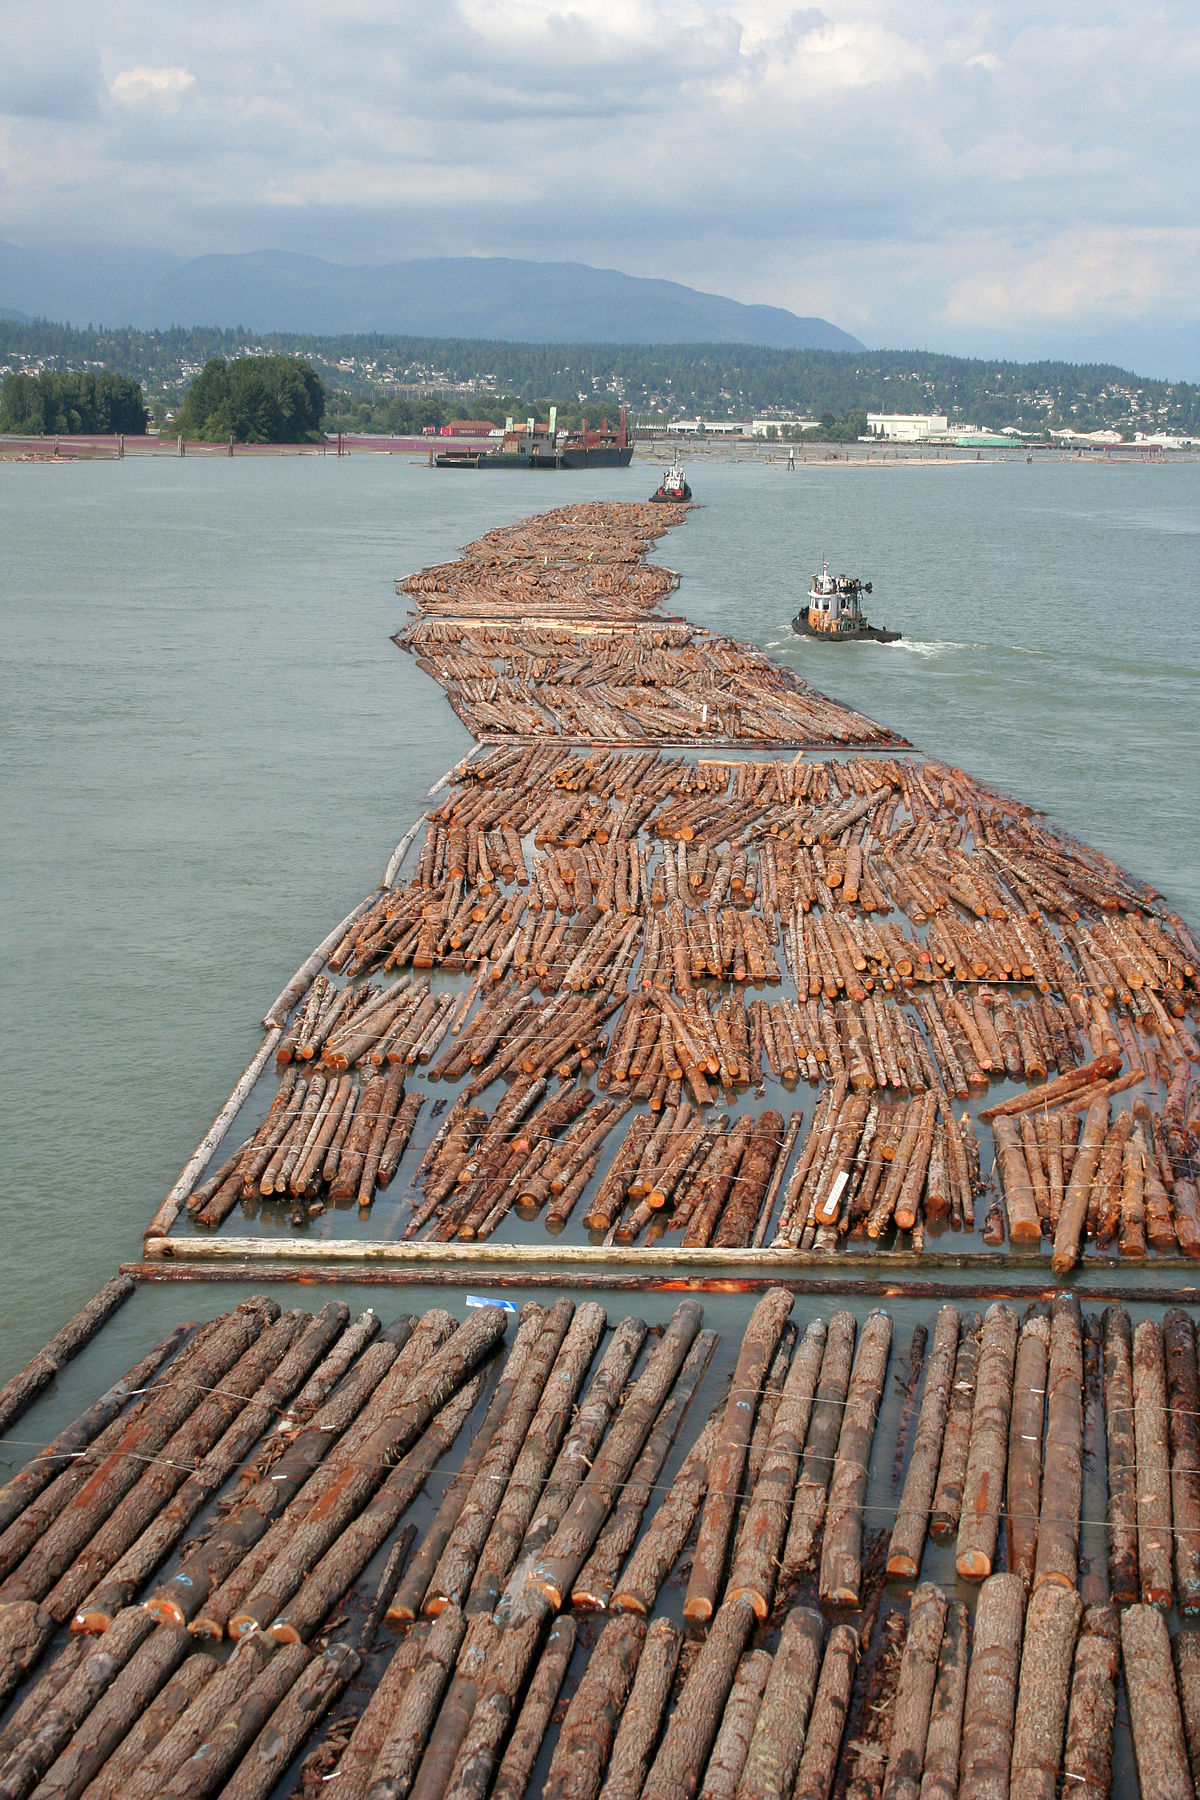
\includegraphics[scale=0.05]{0-figs/parallelization}
\end{frame}


\begin{frame}{Implementation}
  \begin{block}{Right hindsight?}
    \begin{enumerate}
    \item Use the database as much as possible 
    \item Use Views instead of actual storage (so the database can
      handle it in memory)
    \item Allow parallel processing (24 worker threads)
    \end{enumerate}
  \end{block}
  \begin{block}{Actual Implementation}
    \begin{enumerate}
    \item Python 3.5 (main API)
    \item PostgreSQL 9.6
    \end{enumerate}
  \end{block}
  \begin{block}{Show off (1518 lines of python code)}
    \begin{enumerate}
    \item SAT Solver 72 lines
    \item \#SAT Solver 94 lines
    \item Vertex Cover 199 lines
    \end{enumerate}
  \end{block}
\end{frame}


\begin{frame}{How does the Python code look like?}
  \centering
  \resizebox{.9\linewidth}{!}{%
    \lstinputlisting[language=Python]{2-includes/listing.py}
    % 
  }
\end{frame}


\newcommand{\inacc}[1]{\ensuremath{\diamond{}}#1}
\newcommand{\gpusatnu}{gpuSAT2}
\newcommand{\gpusatone}{gpuSAT1}
\newcommand{\gpusatnuv}[1]{gpuSAT2(#1)}

\begin{frame}{Experimental Work}
  \bigskip
  \begin{block}{Instances}
    \begin{itemize}
    \item ~1400 instances from public benchmarks
    \end{itemize}
  \end{block}
  \begin{block}{Limits}
    \begin{itemize}
    \item Cannot expect to solve instances of high treewidth
    \end{itemize}
  \end{block}
  \begin{block}{Setting (Runtime Comparison)}
    \begin{itemize}
    \item Take recent solvers.
    \item Consider Wallclock
    \end{itemize}
  \end{block}
\end{frame}


\begin{frame}{\#SAT: Width \bcite{FHZisser'19}}
  \bigskip\bigskip%
  {\centering
    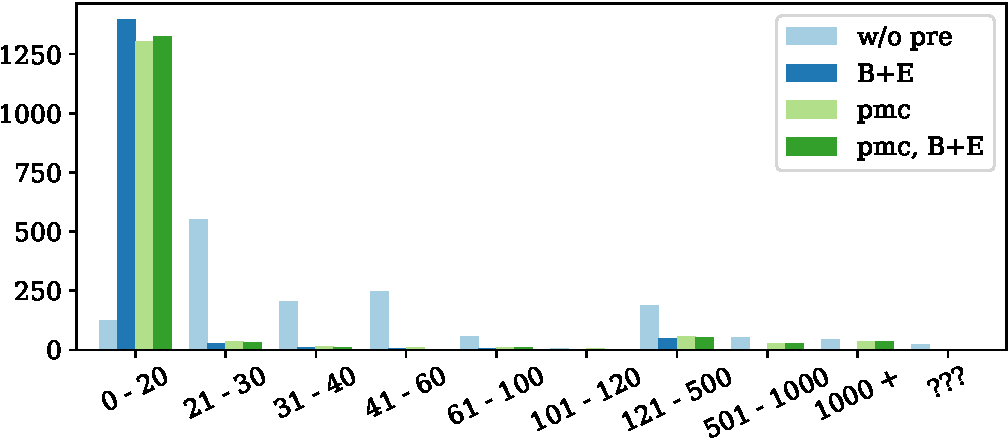
\includegraphics[width=.90\columnwidth]{1-plots/plot_Width.pdf}}\\
\end{frame}



\begin{frame}[shrink=1]{\#SAT (Runtime)}
  \vspace{-1em}\\
  ~\hspace{4em}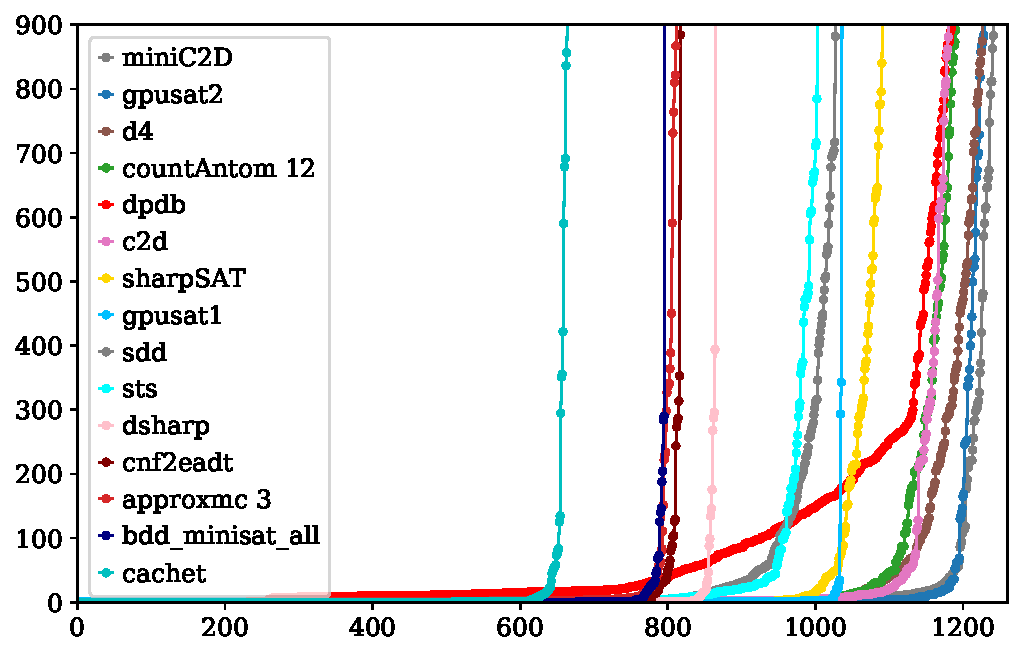
\includegraphics[width=1\columnwidth]{1-plots/plot_pmc.pdf}
\end{frame}


\begin{frame}{Experimental Work (Runtime Disclaimer)}
  \begin{block}{Questionable Setting?}
    Aren't you comparing apples and oranges? YES.
  \end{block}
  \begin{block}{Problems of the Setting}
    \begin{itemize}
    \item We compare on different hardware
    \item Wallclock is unfair
    \item[] Usually user is interested in getting things done
      quickly (+ fairly cheap)
    \item[$\Ra$] Power consumption (Joule) and price of investment
      better measure\\ (BUT not accessible with the current framework)
    \item Parallel vs. sequential: No excuse, sorry
    \end{itemize}
  \end{block}
\end{frame}



\begin{frame}{Summary}
  \begin{block}{Contributions}
    \begin{itemize}
    \item Python framework to implement DPs
    \item Use SQL to specify algorithm
    \item Exploit modern database systems
    \item Framework is surprisingly competitive
    \end{itemize}
  \end{block}
  \begin{block}{Benchmark: Comparing apples and oranges}
    BUT: you compare parallel and sequential solvers.
    \begin{enumerate}
    \item We run on cheap consumer hardware (200\$)
    \item Cannot measure speedup due to OpenCL/display driver limitations\\
      $\Rightarrow$ migrate to cuda
    \end{enumerate}
  \end{block}
\end{frame}

\begin{frame}{Summary cont.}
  \begin{block}{Take Home Messages}
    \begin{enumerate}
    \item Parameterized Algorithms can work\\
      (Preprocessing is key; writing down DPs sucks less)
    \item Download at \url{github.com/hmarkus/dp on dbs.}
    \item Does it ``work'' for SAT? $\Rightarrow$ we don't expect so.
    \end{enumerate}
  \end{block}
  
  \begin{block}{Future Work}
    \begin{itemize}
    \item Postgres 12 / other DBMS
    \item Lift quantified Boolean formulas / projected model counting 
    \end{itemize}
  \end{block}
  \vspace{-0.5em}
  \only<2>{
    \centering
    \alert{%
    Thanks for listening!
    %
    }\medskip\\
    
    % {\color{red}
    %   Advertisement:\\
    %   PACE-2019 (vertex cover and hypertree decompositions)\\
    % {\footnotesize{}GitHub:daajoe/\{benchmark-tool,fhtd,trellis\}}}
    
    %
    \bigskip
    %
  }
  %\alert{Who is interested in collaborating?}
  
  Sponsors: FWF Y698 \& P26696
\end{frame}


\begin{frame}{References}
  \hangpara{5em}{1}[AMW'17]: Abseher, Musliu, Woltran. htd -- A Free,
  Open-Source Framework for (Customized) Tree Decompositions and
  Beyond. CPAIOR'17. 2017. doi: 10.1007/978-3-319-59776-8\_30

  \hangpara{5em}{1}[FHWZ'18]: Fichte, Hecher, Woltran, Zisser. Weighted
  Model Counting on the {GPU} by Exploiting Small
  Treewidth. ESA'18. 2018. doi: 10.4230/LIPIcs.ESA.2018.28

  \hangpara{4.5em}{1}[FHZ'19]: Fichte, Hecher, Zisser. gpusat2 -- An
  Improved GPU Model Counter. CP 2019.

  \hangpara{8.5em}{1}[SamerSzeider'10]: Samer, Szeider. Algorithms for
  propositional model counting. JDA. 2010. doi:
  10.1016/j.jda.2009.06.002
  \bigskip\bigskip

  gpusat is available at: \url{https://github.com/daajoe/gpusat}
\end{frame}


% \begin{frame}[label=questions,noframenumbering]{}
%   \bigskip
%   \bigskip
%   \bigskip
%   \bigskip
%   \bigskip
%   \bigskip
%   \bigskip
%   \begin{center}
%     \alert{\Huge Questions?}
%   \end{center}
%   \bigskip
%   \bigskip
%   \bigskip
%   \bigskip
%   \bigskip
%   \bigskip  
%   \bigskip  
%   \bigskip  
%  \hfill\hyperlink{backup_slides<1>}{\beamergotobutton{Backup Slides}}
% \end{frame}


\beginbackup
\subsection{Backup}


\begin{frame}[label=questions,noframenumbering]{}
  \bigskip
  \bigskip
  \bigskip
  \bigskip
  \bigskip
  \bigskip
  \bigskip
  \begin{center}
    \alert{\Huge Backup Slides}
  \end{center}
  \bigskip
  \bigskip
  \bigskip
  \bigskip
  \bigskip
  \bigskip  
  \bigskip  
  \bigskip  
\end{frame}

\begin{frame}{Experiments (Setup)}
  \begin{block}{Hardware}
    \begin{itemize}
    \item non-GPU solving: cluster of 9 nodes; each two E5-2650
      CPUs (12cores) 2.2 GHz, 256 GB RAM; disabled HT, kernel~4.4
    \item GPU-solving: i3-3245 3.4 GHz; 16 GB RAM; GPU: Sapphire Pulse
      ITX Radeon RX 570 GPU; 1.24 GHz with 32 compute units, 2048
      shader units, 4GB VRAM
    \end{itemize}
  \end{block}
\end{frame}


\begin{frame}[label=algorithm]{Algorithm for Primal Graph}
  \resizebox{0.8\textwidth}{!}{%
    \centering
     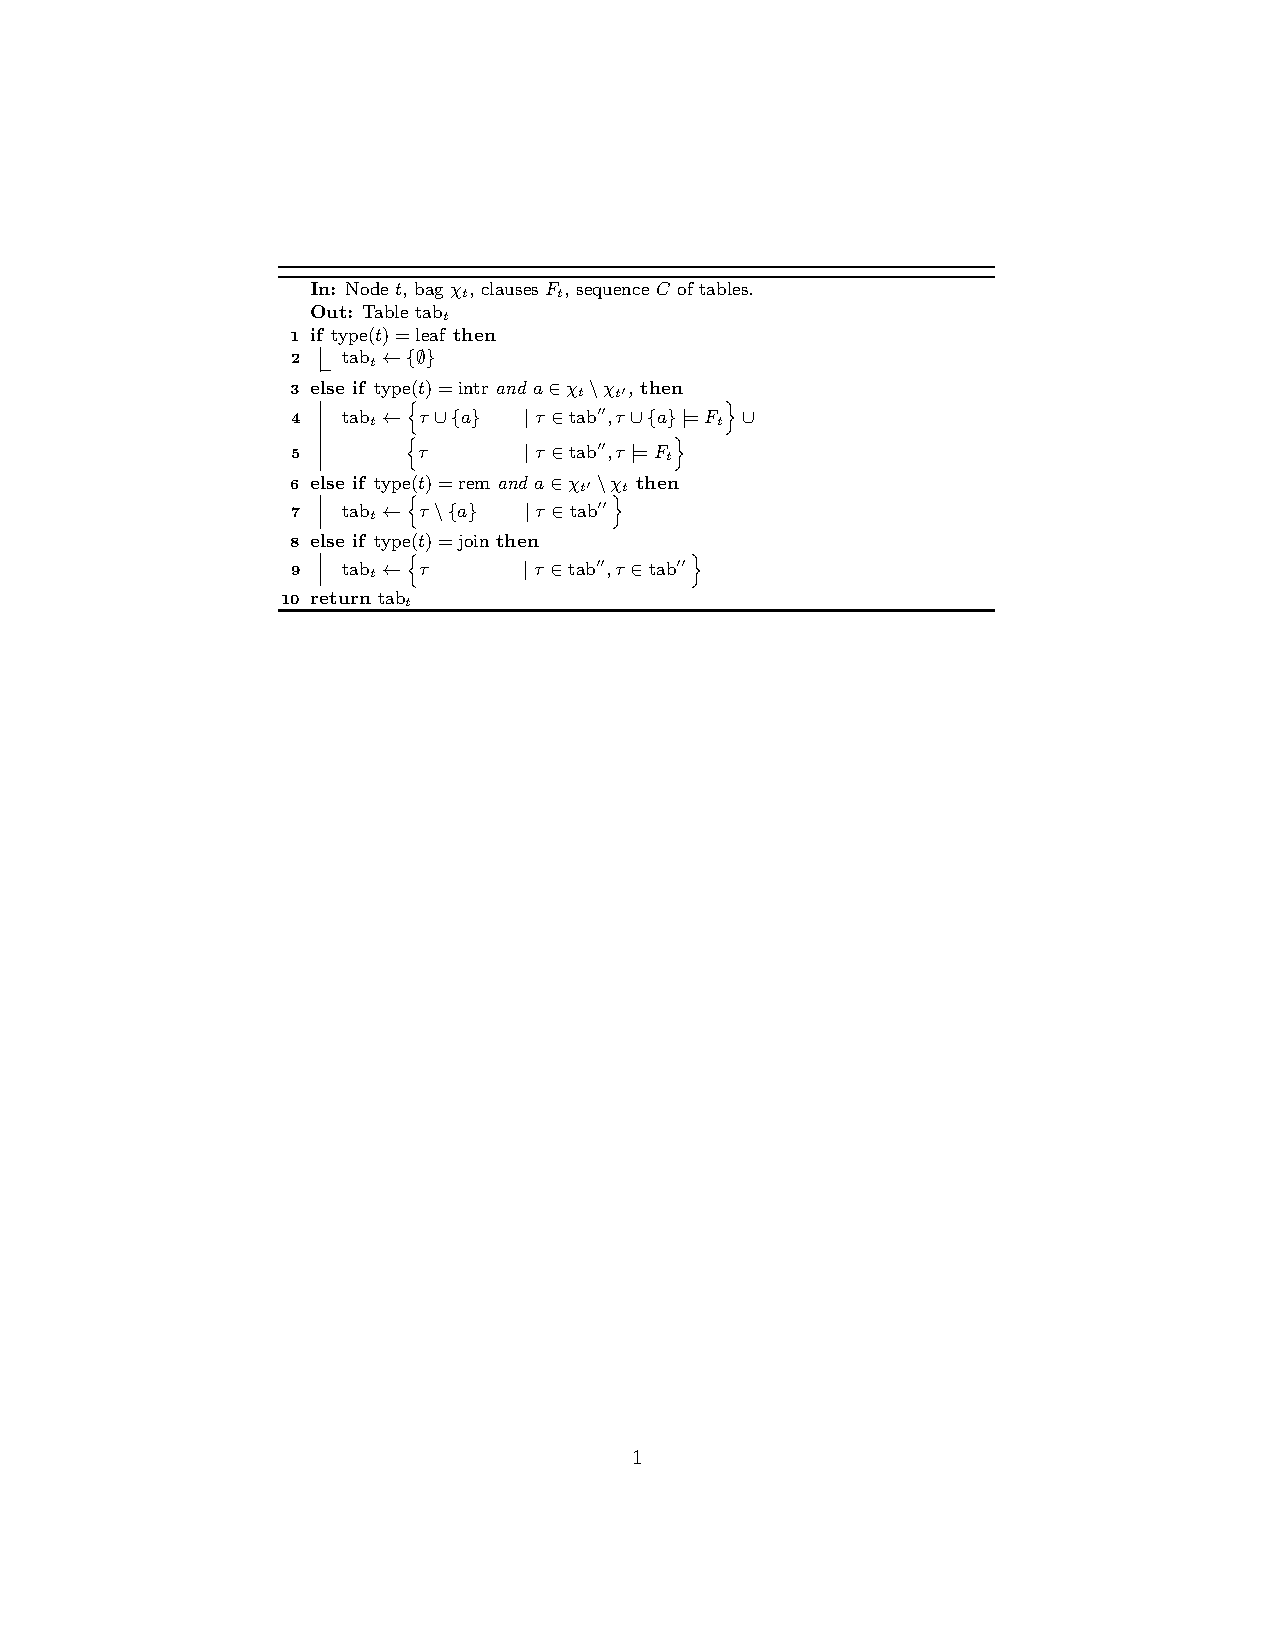
\includegraphics[trim={3.5cm 15cm 8cm 4cm},clip]{2-includes/sat_algo.pdf}
   }
\end{frame}



\backupend

\end{document}

%%% Local Variables:
%%% mode: latex
%%% TeX-engine: xetex
%%% TeX-master: t
%%% End: